\documentclass[twoside]{book}

% Packages required by doxygen
\usepackage{fixltx2e}
\usepackage{calc}
\usepackage{doxygen}
\usepackage[export]{adjustbox} % also loads graphicx
\usepackage{graphicx}
\usepackage[utf8]{inputenc}
\usepackage{makeidx}
\usepackage{multicol}
\usepackage{multirow}
\PassOptionsToPackage{warn}{textcomp}
\usepackage{textcomp}
\usepackage[nointegrals]{wasysym}
\usepackage[table]{xcolor}

% Font selection
\usepackage[T1]{fontenc}
\usepackage[scaled=.90]{helvet}
\usepackage{courier}
\usepackage{amssymb}
\usepackage{sectsty}
\renewcommand{\familydefault}{\sfdefault}
\allsectionsfont{%
  \fontseries{bc}\selectfont%
  \color{darkgray}%
}
\renewcommand{\DoxyLabelFont}{%
  \fontseries{bc}\selectfont%
  \color{darkgray}%
}
\newcommand{\+}{\discretionary{\mbox{\scriptsize$\hookleftarrow$}}{}{}}

% Page & text layout
\usepackage{geometry}
\geometry{%
  a4paper,%
  top=2.5cm,%
  bottom=2.5cm,%
  left=2.5cm,%
  right=2.5cm%
}
\tolerance=750
\hfuzz=15pt
\hbadness=750
\setlength{\emergencystretch}{15pt}
\setlength{\parindent}{0cm}
\setlength{\parskip}{0.2cm}
\makeatletter
\renewcommand{\paragraph}{%
  \@startsection{paragraph}{4}{0ex}{-1.0ex}{1.0ex}{%
    \normalfont\normalsize\bfseries\SS@parafont%
  }%
}
\renewcommand{\subparagraph}{%
  \@startsection{subparagraph}{5}{0ex}{-1.0ex}{1.0ex}{%
    \normalfont\normalsize\bfseries\SS@subparafont%
  }%
}
\makeatother

% Headers & footers
\usepackage{fancyhdr}
\pagestyle{fancyplain}
\fancyhead[LE]{\fancyplain{}{\bfseries\thepage}}
\fancyhead[CE]{\fancyplain{}{}}
\fancyhead[RE]{\fancyplain{}{\bfseries\leftmark}}
\fancyhead[LO]{\fancyplain{}{\bfseries\rightmark}}
\fancyhead[CO]{\fancyplain{}{}}
\fancyhead[RO]{\fancyplain{}{\bfseries\thepage}}
\fancyfoot[LE]{\fancyplain{}{}}
\fancyfoot[CE]{\fancyplain{}{}}
\fancyfoot[RE]{\fancyplain{}{\bfseries\scriptsize Generated by Doxygen }}
\fancyfoot[LO]{\fancyplain{}{\bfseries\scriptsize Generated by Doxygen }}
\fancyfoot[CO]{\fancyplain{}{}}
\fancyfoot[RO]{\fancyplain{}{}}
\renewcommand{\footrulewidth}{0.4pt}
\renewcommand{\chaptermark}[1]{%
  \markboth{#1}{}%
}
\renewcommand{\sectionmark}[1]{%
  \markright{\thesection\ #1}%
}

% Indices & bibliography
\usepackage{natbib}
\usepackage[titles]{tocloft}
\setcounter{tocdepth}{3}
\setcounter{secnumdepth}{5}
\makeindex

% Hyperlinks (required, but should be loaded last)
\usepackage{ifpdf}
\ifpdf
  \usepackage[pdftex,pagebackref=true]{hyperref}
\else
  \usepackage[ps2pdf,pagebackref=true]{hyperref}
\fi
\hypersetup{%
  colorlinks=true,%
  linkcolor=blue,%
  citecolor=blue,%
  unicode%
}

% Custom commands
\newcommand{\clearemptydoublepage}{%
  \newpage{\pagestyle{empty}\cleardoublepage}%
}

\usepackage{caption}
\captionsetup{labelsep=space,justification=centering,font={bf},singlelinecheck=off,skip=4pt,position=top}

%===== C O N T E N T S =====

\begin{document}

% Titlepage & ToC
\hypersetup{pageanchor=false,
             bookmarksnumbered=true,
             pdfencoding=unicode
            }
\pagenumbering{roman}
\begin{titlepage}
\vspace*{7cm}
\begin{center}%
{\Large P\+C\+SC Nonlinear Systems Project }\\
\vspace*{1cm}
{\large Generated by Doxygen 1.8.11}\\
\end{center}
\end{titlepage}
\clearemptydoublepage
\tableofcontents
\clearemptydoublepage
\pagenumbering{arabic}
\hypersetup{pageanchor=true}

%--- Begin generated contents ---
\chapter{Hierarchical Index}
\section{Class Hierarchy}
This inheritance list is sorted roughly, but not completely, alphabetically\+:\begin{DoxyCompactList}
\item \contentsline{section}{Aitken}{\pageref{class_aitken}}{}
\item \contentsline{section}{Equations\+Control}{\pageref{class_equations_control}}{}
\begin{DoxyCompactList}
\item \contentsline{section}{Equations}{\pageref{class_equations}}{}
\begin{DoxyCompactList}
\item \contentsline{section}{Equation\+Tools}{\pageref{class_equation_tools}}{}
\item \contentsline{section}{Gauss}{\pageref{class_gauss}}{}
\item \contentsline{section}{Jacobian}{\pageref{class_jacobian}}{}
\end{DoxyCompactList}
\end{DoxyCompactList}
\item \contentsline{section}{Nonlinear\+Solver}{\pageref{class_nonlinear_solver}}{}
\begin{DoxyCompactList}
\item \contentsline{section}{Bisection}{\pageref{class_bisection}}{}
\item \contentsline{section}{Chord}{\pageref{class_chord}}{}
\item \contentsline{section}{Fixed\+Point}{\pageref{class_fixed_point}}{}
\item \contentsline{section}{Newton}{\pageref{class_newton}}{}
\end{DoxyCompactList}
\item \contentsline{section}{Test\+Suit}{\pageref{class_test_suit}}{}
\end{DoxyCompactList}

\chapter{Class Index}
\section{Class List}
Here are the classes, structs, unions and interfaces with brief descriptions\+:\begin{DoxyCompactList}
\item\contentsline{section}{\hyperlink{class_aitken}{Aitken} \\*\hyperlink{_aitken_8hpp_source}{Aitken.\+hpp} }{\pageref{class_aitken}}{}
\item\contentsline{section}{\hyperlink{class_bisection}{Bisection} \\*\hyperlink{_bisection_8hpp_source}{Bisection.\+hpp} }{\pageref{class_bisection}}{}
\item\contentsline{section}{\hyperlink{class_chord}{Chord} \\*\hyperlink{_chord_8hpp_source}{Chord.\+hpp} }{\pageref{class_chord}}{}
\item\contentsline{section}{\hyperlink{class_equations_control}{Equations\+Control} \\*Equations\+Control.\+hpp }{\pageref{class_equations_control}}{}
\item\contentsline{section}{\hyperlink{class_equation_tools}{Equation\+Tools} \\*Equation\+Tools.\+hpp }{\pageref{class_equation_tools}}{}
\item\contentsline{section}{\hyperlink{class_expression}{Expression} \\*\hyperlink{_expression_8hpp_source}{Expression.\+hpp} }{\pageref{class_expression}}{}
\item\contentsline{section}{\hyperlink{class_expression_system}{Expression\+System} \\*\hyperlink{_expression_system_8hpp_source}{Expression\+System.\+hpp} }{\pageref{class_expression_system}}{}
\item\contentsline{section}{\hyperlink{class_fixed_point}{Fixed\+Point} \\*\hyperlink{_fixed_point_8hpp_source}{Fixed\+Point.\+hpp} }{\pageref{class_fixed_point}}{}
\item\contentsline{section}{\hyperlink{class_gauss}{Gauss} \\*Gauss.\+hpp }{\pageref{class_gauss}}{}
\item\contentsline{section}{\hyperlink{class_helper}{Helper} }{\pageref{class_helper}}{}
\item\contentsline{section}{\hyperlink{class_initial_vector}{Initial\+Vector} }{\pageref{class_initial_vector}}{}
\item\contentsline{section}{\hyperlink{class_newton}{Newton} \\*\hyperlink{_newton_8hpp_source}{Newton.\+hpp} }{\pageref{class_newton}}{}
\item\contentsline{section}{\hyperlink{class_newton_system}{Newton\+System} }{\pageref{class_newton_system}}{}
\item\contentsline{section}{\hyperlink{class_nonlinear_solver}{Nonlinear\+Solver} \\*\hyperlink{_nonlinear_solver_8hpp_source}{Nonlinear\+Solver.\+hpp} }{\pageref{class_nonlinear_solver}}{}
\item\contentsline{section}{\hyperlink{class_nonlinear_systems_solver}{Nonlinear\+Systems\+Solver} \\*\hyperlink{_nonlinear_systems_solver_8hpp_source}{Nonlinear\+Systems\+Solver.\+hpp} }{\pageref{class_nonlinear_systems_solver}}{}
\item\contentsline{section}{\hyperlink{class_test_suit}{Test\+Suit} }{\pageref{class_test_suit}}{}
\end{DoxyCompactList}

\chapter{File Index}
\section{File List}
Here is a list of all documented files with brief descriptions\+:\begin{DoxyCompactList}
\item\contentsline{section}{code/{\bfseries Aitken.\+hpp} }{\pageref{_aitken_8hpp}}{}
\item\contentsline{section}{code/{\bfseries Bisection.\+hpp} }{\pageref{_bisection_8hpp}}{}
\item\contentsline{section}{code/{\bfseries Chord.\+hpp} }{\pageref{_chord_8hpp}}{}
\item\contentsline{section}{code/{\bfseries Equations\+Control.\+h} }{\pageref{_equations_control_8h}}{}
\item\contentsline{section}{code/{\bfseries Equation\+Tools.\+h} }{\pageref{_equation_tools_8h}}{}
\item\contentsline{section}{code/{\bfseries Exception.\+hpp} }{\pageref{_exception_8hpp}}{}
\item\contentsline{section}{code/{\bfseries Expression.\+hpp} }{\pageref{_expression_8hpp}}{}
\item\contentsline{section}{code/{\bfseries Expression\+System.\+hpp} }{\pageref{_expression_system_8hpp}}{}
\item\contentsline{section}{code/{\bfseries Fixed\+Point.\+hpp} }{\pageref{_fixed_point_8hpp}}{}
\item\contentsline{section}{code/{\bfseries Gauss.\+h} }{\pageref{_gauss_8h}}{}
\item\contentsline{section}{code/{\bfseries Helper.\+hpp} }{\pageref{_helper_8hpp}}{}
\item\contentsline{section}{code/{\bfseries Initial\+Vector.\+hpp} }{\pageref{_initial_vector_8hpp}}{}
\item\contentsline{section}{code/{\bfseries Newton.\+hpp} }{\pageref{_newton_8hpp}}{}
\item\contentsline{section}{code/{\bfseries Newton\+System.\+hpp} }{\pageref{_newton_system_8hpp}}{}
\item\contentsline{section}{code/{\bfseries Nonlinear\+Solver.\+hpp} }{\pageref{_nonlinear_solver_8hpp}}{}
\item\contentsline{section}{code/{\bfseries Nonlinear\+Systems\+Solver.\+hpp} }{\pageref{_nonlinear_systems_solver_8hpp}}{}
\item\contentsline{section}{code/\hyperlink{string_8hpp}{string.\+hpp} }{\pageref{string_8hpp}}{}
\item\contentsline{section}{code/{\bfseries Tests.\+h} }{\pageref{_tests_8h}}{}
\end{DoxyCompactList}

\chapter{Class Documentation}
\hypertarget{class_aitken}{}\section{Aitken Class Reference}
\label{class_aitken}\index{Aitken@{Aitken}}


\hyperlink{_aitken_8hpp_source}{Aitken.\+hpp}.  




{\ttfamily \#include $<$Aitken.\+hpp$>$}

Inheritance diagram for Aitken\+:\begin{figure}[H]
\begin{center}
\leavevmode
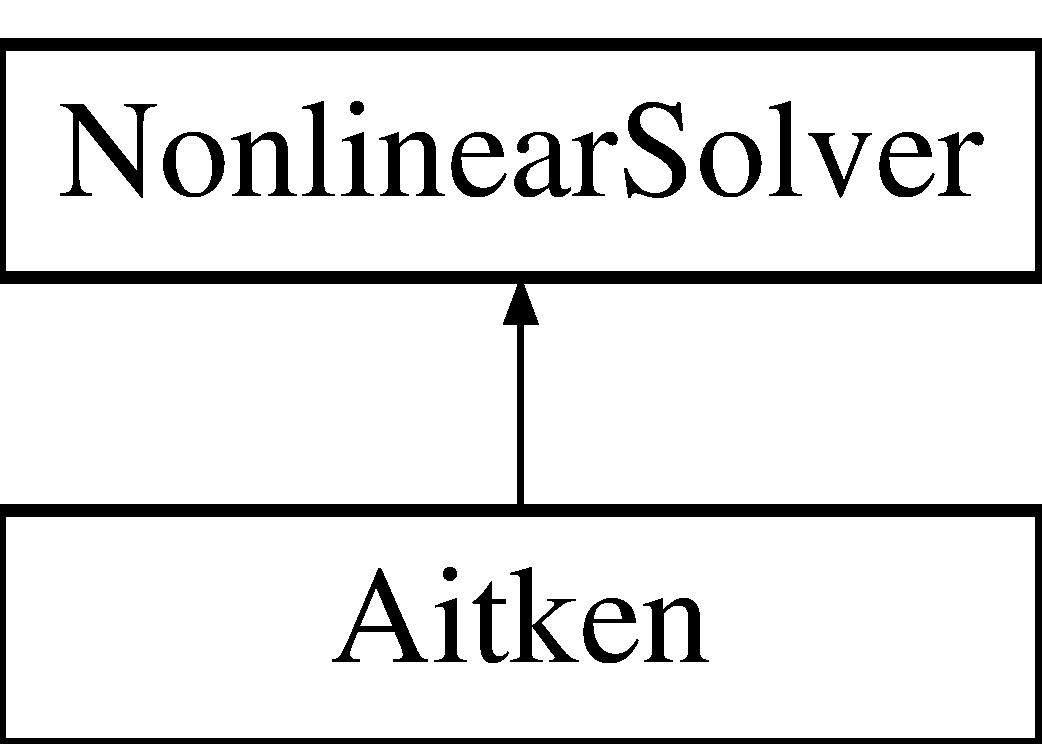
\includegraphics[height=2.000000cm]{class_aitken}
\end{center}
\end{figure}
\subsection*{Public Member Functions}
\begin{DoxyCompactItemize}
\item 
\hyperlink{class_aitken_a4a67b211a085f7acbc059575427b543b}{Aitken} (\hyperlink{class_expression}{Expression} \&equation, double initial, double tolerance, int max\+Iter, bool verbosity)
\item 
virtual \hyperlink{class_aitken_a1d89b3f0a4748c6aa71fa6324707f93b}{$\sim$\+Aitken} ()\hypertarget{class_aitken_a1d89b3f0a4748c6aa71fa6324707f93b}{}\label{class_aitken_a1d89b3f0a4748c6aa71fa6324707f93b}

\begin{DoxyCompactList}\small\item\em A virtual destructor for the \hyperlink{class_aitken}{Aitken} method. \end{DoxyCompactList}\item 
double \hyperlink{class_aitken_a2fc0237c34ae1d84e02f92d1d28614e9}{solve} ()
\end{DoxyCompactItemize}
\subsection*{Additional Inherited Members}


\subsection{Detailed Description}
\hyperlink{_aitken_8hpp_source}{Aitken.\+hpp}. 

A class constructing an object capable of solving nonlinear systems with the \hyperlink{class_aitken}{Aitken} method. \begin{DoxyAuthor}{Author}
Jaquier, Michael \href{mailto:michael.jaquier@epfl.ch}{\tt michael.\+jaquier@epfl.\+ch} 

Lorkowski, Alexander \href{mailto:alexander.lorkowski@epfl.ch}{\tt alexander.\+lorkowski@epfl.\+ch} 
\end{DoxyAuthor}
\begin{DoxyVersion}{Version}
1.\+0 
\end{DoxyVersion}
\begin{DoxyDate}{Date}
10 December 2016 
\end{DoxyDate}
\begin{DoxyRemark}{Remarks}
Ecole Polytechnic Federal de Lausanne (E\+P\+FL) 

M\+A\+T\+H-\/458 Programming Concepts in Scientific Computing 
\end{DoxyRemark}


\subsection{Constructor \& Destructor Documentation}
\index{Aitken@{Aitken}!Aitken@{Aitken}}
\index{Aitken@{Aitken}!Aitken@{Aitken}}
\subsubsection[{\texorpdfstring{Aitken(\+Expression \&equation, double initial, double tolerance, int max\+Iter, bool verbosity)}{Aitken(Expression &equation, double initial, double tolerance, int maxIter, bool verbosity)}}]{\setlength{\rightskip}{0pt plus 5cm}Aitken\+::\+Aitken (
\begin{DoxyParamCaption}
\item[{{\bf Expression} \&}]{equation, }
\item[{double}]{initial, }
\item[{double}]{tolerance, }
\item[{int}]{max\+Iter, }
\item[{bool}]{verbosity}
\end{DoxyParamCaption}
)}\hypertarget{class_aitken_a4a67b211a085f7acbc059575427b543b}{}\label{class_aitken_a4a67b211a085f7acbc059575427b543b}
A constructor to instantiate variables for the \hyperlink{class_aitken}{Aitken} method.


\begin{DoxyParams}{Parameters}
{\em equation} & An object of the \hyperlink{class_expression}{Expression} class that contains the mathematical expression for the class to evaluate. \\
\hline
{\em initial} & The initial guess of the solution to the equation. \\
\hline
{\em tolerance} & The tolerance value. The method stops once the residual errors fall below this value. \\
\hline
{\em max\+Iter} & The maximum number of iterations. The method stops once this number is reached. \\
\hline
{\em verbosity} & Set to true to print all intermediate and final results onto the console. \\
\hline
\end{DoxyParams}


\subsection{Member Function Documentation}
\index{Aitken@{Aitken}!solve@{solve}}
\index{solve@{solve}!Aitken@{Aitken}}
\subsubsection[{\texorpdfstring{solve()}{solve()}}]{\setlength{\rightskip}{0pt plus 5cm}double Aitken\+::solve (
\begin{DoxyParamCaption}
{}
\end{DoxyParamCaption}
)\hspace{0.3cm}{\ttfamily [virtual]}}\hypertarget{class_aitken_a2fc0237c34ae1d84e02f92d1d28614e9}{}\label{class_aitken_a2fc0237c34ae1d84e02f92d1d28614e9}
A function when called returns the solution to the \hyperlink{class_aitken}{Aitken} Method.

\begin{DoxyReturn}{Returns}
The solution to the \hyperlink{class_aitken}{Aitken} Method. 
\end{DoxyReturn}


Implements \hyperlink{class_nonlinear_solver_a72180277586bd7ec915cc4a806f62bb9}{Nonlinear\+Solver}.



The documentation for this class was generated from the following files\+:\begin{DoxyCompactItemize}
\item 
code/Aitken.\+hpp\item 
code/Aitken.\+cpp\end{DoxyCompactItemize}

\hypertarget{class_bisection}{}\section{Bisection Class Reference}
\label{class_bisection}\index{Bisection@{Bisection}}


\hyperlink{_bisection_8hpp_source}{Bisection.\+hpp}.  




{\ttfamily \#include $<$Bisection.\+hpp$>$}

Inheritance diagram for Bisection\+:\begin{figure}[H]
\begin{center}
\leavevmode
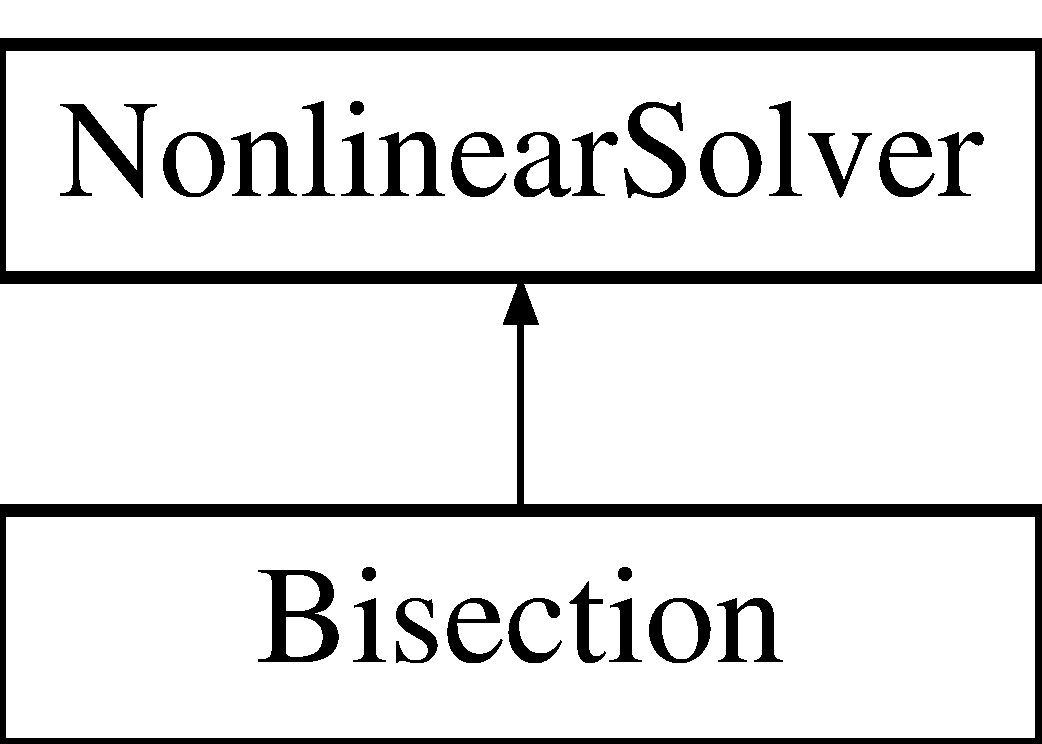
\includegraphics[height=2.000000cm]{class_bisection}
\end{center}
\end{figure}
\subsection*{Public Member Functions}
\begin{DoxyCompactItemize}
\item 
virtual \hyperlink{class_bisection_a44d6c2c0a557a6540980c23ef7eaa6a4}{$\sim$\+Bisection} ()\hypertarget{class_bisection_a44d6c2c0a557a6540980c23ef7eaa6a4}{}\label{class_bisection_a44d6c2c0a557a6540980c23ef7eaa6a4}

\begin{DoxyCompactList}\small\item\em A virtual destructor for the \hyperlink{class_bisection}{Bisection} method. \end{DoxyCompactList}\item 
\hyperlink{class_bisection_afef6fa8f828ffa4f46e26189425421bf}{Bisection} (\hyperlink{class_expression}{Expression} \&equation, double initial, double tolerance, int max\+Iter, bool verbosity)
\item 
\hyperlink{class_bisection_a38ccdd59524e49ec73ee437f9daa5033}{Bisection} (\hyperlink{class_expression}{Expression} \&equation, double initial, double tolerance, int max\+Iter, bool verbosity, double lower\+Bound, double upper\+Bound)
\item 
double \hyperlink{class_bisection_a14e36ab0143cf54dc71f2c9da238fe15}{solve} ()
\end{DoxyCompactItemize}
\subsection*{Additional Inherited Members}


\subsection{Detailed Description}
\hyperlink{_bisection_8hpp_source}{Bisection.\+hpp}. 

A class constructing an object capable of solving nonlinear systems with the \hyperlink{class_bisection}{Bisection} method. \begin{DoxyAuthor}{Author}
Jaquier, Michael \href{mailto:michael.jaquier@epfl.ch}{\tt michael.\+jaquier@epfl.\+ch} 

Lorkowski, Alexander \href{mailto:alexander.lorkowski@epfl.ch}{\tt alexander.\+lorkowski@epfl.\+ch} 
\end{DoxyAuthor}
\begin{DoxyVersion}{Version}
1.\+0 
\end{DoxyVersion}
\begin{DoxyDate}{Date}
10 December 2016 
\end{DoxyDate}
\begin{DoxyRemark}{Remarks}
Ecole Polytechnic Federal de Lausanne (E\+P\+FL) 

M\+A\+T\+H-\/458 Programming Concepts in Scientific Computing 
\end{DoxyRemark}


\subsection{Constructor \& Destructor Documentation}
\index{Bisection@{Bisection}!Bisection@{Bisection}}
\index{Bisection@{Bisection}!Bisection@{Bisection}}
\subsubsection[{\texorpdfstring{Bisection(\+Expression \&equation, double initial, double tolerance, int max\+Iter, bool verbosity)}{Bisection(Expression &equation, double initial, double tolerance, int maxIter, bool verbosity)}}]{\setlength{\rightskip}{0pt plus 5cm}Bisection\+::\+Bisection (
\begin{DoxyParamCaption}
\item[{{\bf Expression} \&}]{equation, }
\item[{double}]{initial, }
\item[{double}]{tolerance, }
\item[{int}]{max\+Iter, }
\item[{bool}]{verbosity}
\end{DoxyParamCaption}
)}\hypertarget{class_bisection_afef6fa8f828ffa4f46e26189425421bf}{}\label{class_bisection_afef6fa8f828ffa4f46e26189425421bf}
A constructor to instantiate variables for the \hyperlink{class_bisection}{Bisection} method. The default bound is \mbox{[}-\/1,1\mbox{]}.


\begin{DoxyParams}{Parameters}
{\em equation} & A string that contains the mathematical expression for the class to evaluate. \\
\hline
{\em initial} & The initial guess of the solution to the equation. \\
\hline
{\em tolerance} & The tolerance value. The method stops once the residual errors fall below this value. \\
\hline
{\em max\+Iter} & The maximum number of iterations. The method stops once this number is reached. \\
\hline
{\em verbosity} & Set to true to print all intermediate and final results onto the console. \\
\hline
\end{DoxyParams}
\index{Bisection@{Bisection}!Bisection@{Bisection}}
\index{Bisection@{Bisection}!Bisection@{Bisection}}
\subsubsection[{\texorpdfstring{Bisection(\+Expression \&equation, double initial, double tolerance, int max\+Iter, bool verbosity, double lower\+Bound, double upper\+Bound)}{Bisection(Expression &equation, double initial, double tolerance, int maxIter, bool verbosity, double lowerBound, double upperBound)}}]{\setlength{\rightskip}{0pt plus 5cm}Bisection\+::\+Bisection (
\begin{DoxyParamCaption}
\item[{{\bf Expression} \&}]{equation, }
\item[{double}]{initial, }
\item[{double}]{tolerance, }
\item[{int}]{max\+Iter, }
\item[{bool}]{verbosity, }
\item[{double}]{lower\+Bound, }
\item[{double}]{upper\+Bound}
\end{DoxyParamCaption}
)}\hypertarget{class_bisection_a38ccdd59524e49ec73ee437f9daa5033}{}\label{class_bisection_a38ccdd59524e49ec73ee437f9daa5033}
A constructor to instantiate variables for the \hyperlink{class_bisection}{Bisection} method.


\begin{DoxyParams}{Parameters}
{\em equation} & A string that contains the mathematical expression for the class to evaluate. \\
\hline
{\em initial} & The initial guess of the solution to the equation. \\
\hline
{\em tolerance} & The tolerance value. The method stops once the residual errors fall below this value. \\
\hline
{\em max\+Iter} & The maximum number of iterations. The method stops once this number is reached. \\
\hline
{\em verbosity} & Set to true to print all intermediate and final results onto the console. \\
\hline
{\em lower\+Bound} & The lower bound on the domain where the program looks for the solution. \\
\hline
{\em upper\+Bound} & The upper bound on the domain where the program looks for the solution. \\
\hline
\end{DoxyParams}


\subsection{Member Function Documentation}
\index{Bisection@{Bisection}!solve@{solve}}
\index{solve@{solve}!Bisection@{Bisection}}
\subsubsection[{\texorpdfstring{solve()}{solve()}}]{\setlength{\rightskip}{0pt plus 5cm}double Bisection\+::solve (
\begin{DoxyParamCaption}
{}
\end{DoxyParamCaption}
)\hspace{0.3cm}{\ttfamily [virtual]}}\hypertarget{class_bisection_a14e36ab0143cf54dc71f2c9da238fe15}{}\label{class_bisection_a14e36ab0143cf54dc71f2c9da238fe15}
A function that returns the solution to the \hyperlink{class_bisection}{Bisection} method.

\begin{DoxyReturn}{Returns}
The solution to the \hyperlink{class_bisection}{Bisection} Method. 
\end{DoxyReturn}


Implements \hyperlink{class_nonlinear_solver_a72180277586bd7ec915cc4a806f62bb9}{Nonlinear\+Solver}.



The documentation for this class was generated from the following files\+:\begin{DoxyCompactItemize}
\item 
code/Bisection.\+hpp\item 
code/Bisection.\+cpp\end{DoxyCompactItemize}

\hypertarget{class_chord}{}\section{Chord Class Reference}
\label{class_chord}\index{Chord@{Chord}}


\hyperlink{_chord_8hpp_source}{Chord.\+hpp}.  




{\ttfamily \#include $<$Chord.\+hpp$>$}

Inheritance diagram for Chord\+:\begin{figure}[H]
\begin{center}
\leavevmode
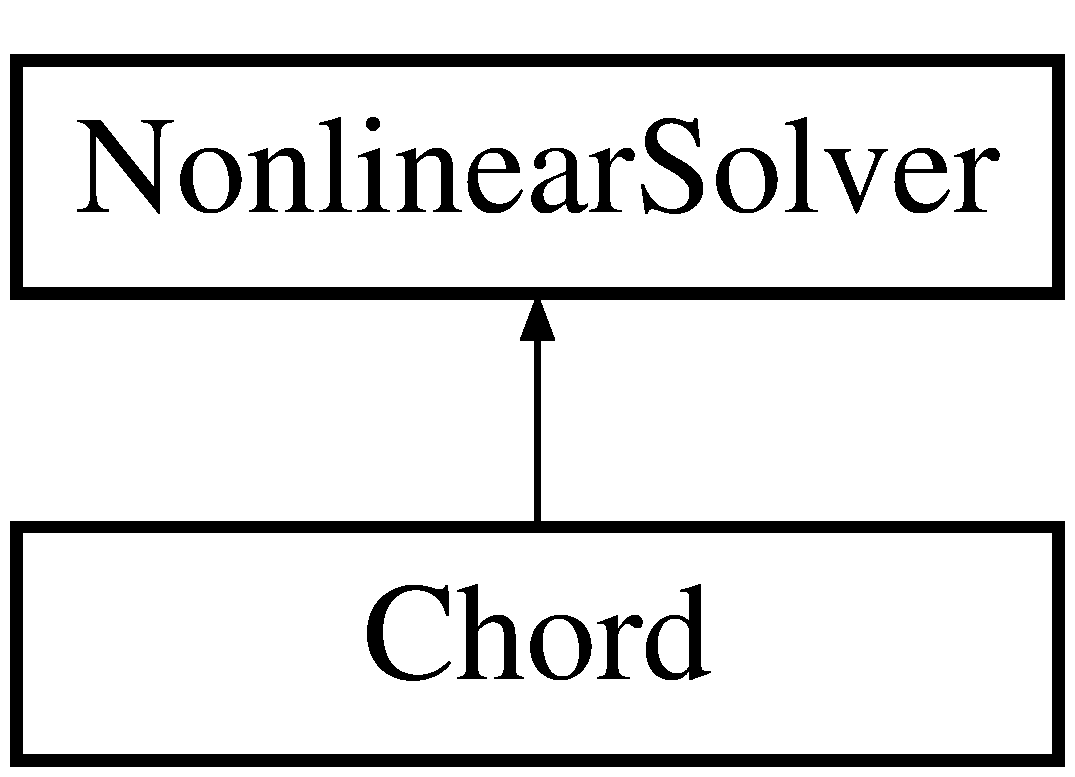
\includegraphics[height=2.000000cm]{class_chord}
\end{center}
\end{figure}
\subsection*{Public Member Functions}
\begin{DoxyCompactItemize}
\item 
\hyperlink{class_chord_a276152dc216ada11e924b9ddac8b6260}{Chord} (\hyperlink{class_expression}{Expression} \&equation, double initial, double tolerance, int max\+Iter, bool verbosity)
\item 
virtual \hyperlink{class_chord_ac1ed7ca66d87b80a1a98e6981b5e6b9e}{$\sim$\+Chord} ()\hypertarget{class_chord_ac1ed7ca66d87b80a1a98e6981b5e6b9e}{}\label{class_chord_ac1ed7ca66d87b80a1a98e6981b5e6b9e}

\begin{DoxyCompactList}\small\item\em A virtual destructor for the \hyperlink{class_chord}{Chord} method. \end{DoxyCompactList}\item 
double \hyperlink{class_chord_a984ae41890e938218b3820ff429ad69e}{solve} ()
\end{DoxyCompactItemize}
\subsection*{Additional Inherited Members}


\subsection{Detailed Description}
\hyperlink{_chord_8hpp_source}{Chord.\+hpp}. 

A class constructing an object capable of solving nonlinear systems with the \hyperlink{class_chord}{Chord} method. \begin{DoxyAuthor}{Author}
Jaquier, Michael \href{mailto:michael.jaquier@epfl.ch}{\tt michael.\+jaquier@epfl.\+ch} 

Lorkowski, Alexander \href{mailto:alexander.lorkowski@epfl.ch}{\tt alexander.\+lorkowski@epfl.\+ch} 
\end{DoxyAuthor}
\begin{DoxyVersion}{Version}
1.\+0 
\end{DoxyVersion}
\begin{DoxyDate}{Date}
10 December 2016 
\end{DoxyDate}
\begin{DoxyRemark}{Remarks}
Ecole Polytechnic Federal de Lausanne (E\+P\+FL) 

M\+A\+T\+H-\/458 Programming Concepts in Scientific Computing 
\end{DoxyRemark}


\subsection{Constructor \& Destructor Documentation}
\index{Chord@{Chord}!Chord@{Chord}}
\index{Chord@{Chord}!Chord@{Chord}}
\subsubsection[{\texorpdfstring{Chord(\+Expression \&equation, double initial, double tolerance, int max\+Iter, bool verbosity)}{Chord(Expression &equation, double initial, double tolerance, int maxIter, bool verbosity)}}]{\setlength{\rightskip}{0pt plus 5cm}Chord\+::\+Chord (
\begin{DoxyParamCaption}
\item[{{\bf Expression} \&}]{equation, }
\item[{double}]{initial, }
\item[{double}]{tolerance, }
\item[{int}]{max\+Iter, }
\item[{bool}]{verbosity}
\end{DoxyParamCaption}
)}\hypertarget{class_chord_a276152dc216ada11e924b9ddac8b6260}{}\label{class_chord_a276152dc216ada11e924b9ddac8b6260}
A constructor to instantiate variables for the \hyperlink{class_chord}{Chord} method.


\begin{DoxyParams}{Parameters}
{\em equation} & An object of the \hyperlink{class_expression}{Expression} class that contains the mathematical expression for the class to evaluate. \\
\hline
{\em initial} & The initial guess of the solution to the equation. \\
\hline
{\em tolerance} & The tolerance value. The method stops once the residual errors fall below this value. \\
\hline
{\em max\+Iter} & The maximum number of iterations. The method stops once this number is reached. \\
\hline
{\em verbosity} & Set to true to print all intermediate and final results onto the console. \\
\hline
\end{DoxyParams}


\subsection{Member Function Documentation}
\index{Chord@{Chord}!solve@{solve}}
\index{solve@{solve}!Chord@{Chord}}
\subsubsection[{\texorpdfstring{solve()}{solve()}}]{\setlength{\rightskip}{0pt plus 5cm}double Chord\+::solve (
\begin{DoxyParamCaption}
{}
\end{DoxyParamCaption}
)\hspace{0.3cm}{\ttfamily [virtual]}}\hypertarget{class_chord_a984ae41890e938218b3820ff429ad69e}{}\label{class_chord_a984ae41890e938218b3820ff429ad69e}
A function that returns the solution to the \hyperlink{class_chord}{Chord} method.

\begin{DoxyReturn}{Returns}
The solution to the \hyperlink{class_chord}{Chord} Method. 
\end{DoxyReturn}


Implements \hyperlink{class_nonlinear_solver_a72180277586bd7ec915cc4a806f62bb9}{Nonlinear\+Solver}.



The documentation for this class was generated from the following files\+:\begin{DoxyCompactItemize}
\item 
code/Chord.\+hpp\item 
code/Chord.\+cpp\end{DoxyCompactItemize}

\hypertarget{class_equations_control}{}\section{Equations\+Control Class Reference}
\label{class_equations_control}\index{Equations\+Control@{Equations\+Control}}


Equations\+Control.\+hpp.  




{\ttfamily \#include $<$Equations\+Control.\+h$>$}



\subsection{Detailed Description}
Equations\+Control.\+hpp. 

A class handling the errors of the exprtk parser. \begin{DoxyAuthor}{Author}
Jaquier, Michael \href{mailto:michael.jaquier@epfl.ch}{\tt michael.\+jaquier@epfl.\+ch} 

Lorkowski, Alexander \href{mailto:alexander.lorkowski@epfl.ch}{\tt alexander.\+lorkowski@epfl.\+ch} 
\end{DoxyAuthor}
\begin{DoxyVersion}{Version}
1.\+0 
\end{DoxyVersion}
\begin{DoxyDate}{Date}
10 December 2016 
\end{DoxyDate}
\begin{DoxyRemark}{Remarks}
Ecole Polytechnic Federal de Lausanne (E\+P\+FL) 

M\+A\+T\+H-\/458 Programming Concepts in Scientific Computing 
\end{DoxyRemark}


The documentation for this class was generated from the following file\+:\begin{DoxyCompactItemize}
\item 
code/Equations\+Control.\+h\end{DoxyCompactItemize}

\hypertarget{class_equation_tools}{}\section{Equation\+Tools Class Reference}
\label{class_equation_tools}\index{Equation\+Tools@{Equation\+Tools}}
Inheritance diagram for Equation\+Tools\+:\begin{figure}[H]
\begin{center}
\leavevmode
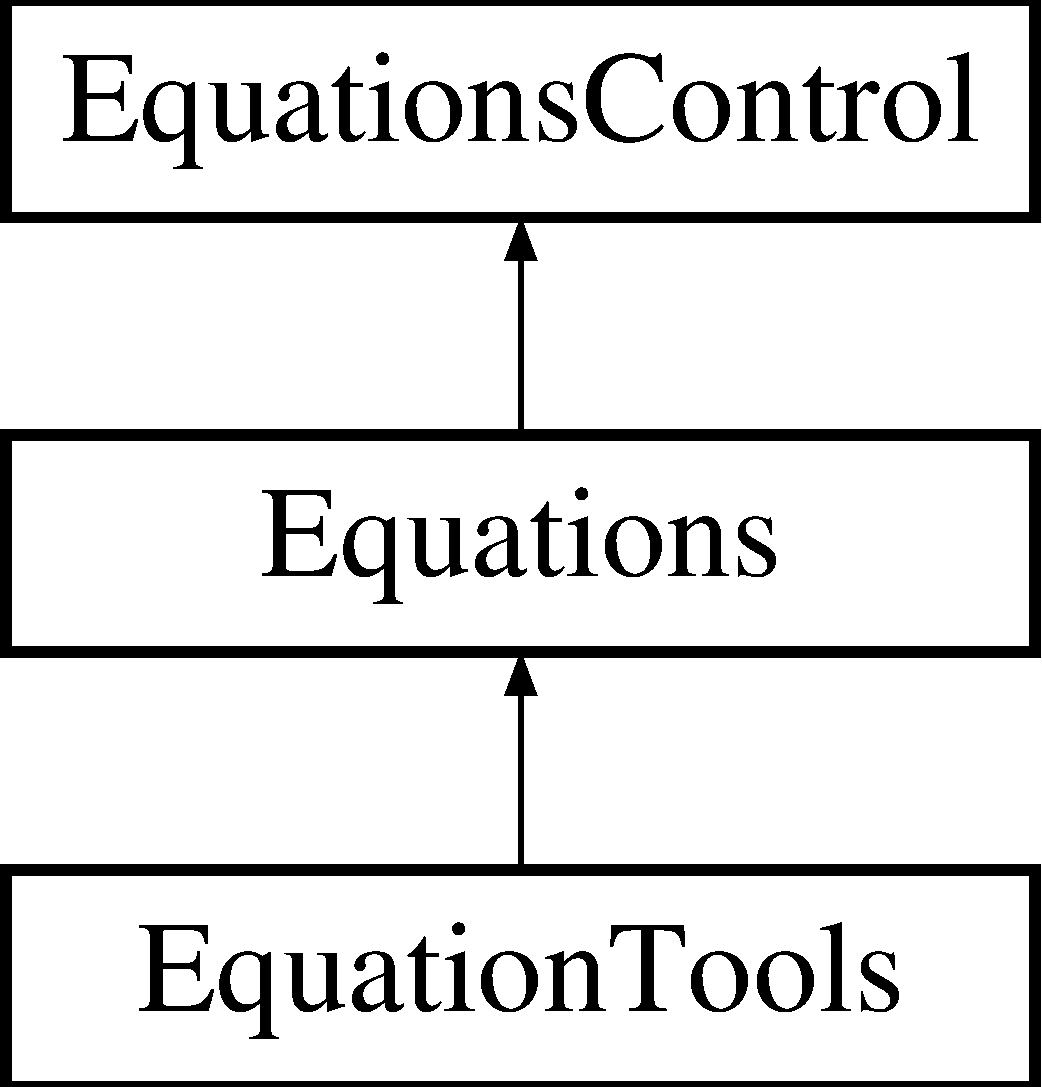
\includegraphics[height=3.000000cm]{class_equation_tools}
\end{center}
\end{figure}
\subsection*{Public Member Functions}
\begin{DoxyCompactItemize}
\item 
std\+::\+\_\+\+\_\+1\+::vector$<$ std\+::\+\_\+\+\_\+1\+::vector$<$ double $>$ $>$ \hyperlink{class_equation_tools_a2400ef03ac5def7120afa962f8a2ec0c}{create\+Minor} (unsigned long size)
\item 
double \hyperlink{class_equation_tools_afba38557ac202d75d3acb90994020f06}{Determinant} (std\+::\+\_\+\+\_\+1\+::vector$<$ std\+::\+\_\+\+\_\+1\+::vector$<$ double $>$$>$ \&M, const int size)
\end{DoxyCompactItemize}
\subsection*{Additional Inherited Members}


\subsection{Member Function Documentation}
\index{Equation\+Tools@{Equation\+Tools}!create\+Minor@{create\+Minor}}
\index{create\+Minor@{create\+Minor}!Equation\+Tools@{Equation\+Tools}}
\subsubsection[{\texorpdfstring{create\+Minor(unsigned long size)}{createMinor(unsigned long size)}}]{\setlength{\rightskip}{0pt plus 5cm}std\+::\+\_\+\+\_\+1\+::vector$<$ std\+::\+\_\+\+\_\+1\+::vector$<$ double $>$ $>$ Equation\+Tools\+::create\+Minor (
\begin{DoxyParamCaption}
\item[{unsigned long}]{size}
\end{DoxyParamCaption}
)}\hypertarget{class_equation_tools_a2400ef03ac5def7120afa962f8a2ec0c}{}\label{class_equation_tools_a2400ef03ac5def7120afa962f8a2ec0c}
Create a vector$<$vector$>$ to be populated later 
\begin{DoxyParams}{Parameters}
{\em size} & -\/ of the Main Vector$<$\+Vector$>$ -\/ 1 \\
\hline
\end{DoxyParams}
\begin{DoxyReturn}{Returns}
A NxN vector$<$vector$>$ of zeros 
\end{DoxyReturn}
\index{Equation\+Tools@{Equation\+Tools}!Determinant@{Determinant}}
\index{Determinant@{Determinant}!Equation\+Tools@{Equation\+Tools}}
\subsubsection[{\texorpdfstring{Determinant(std\+::\+\_\+\+\_\+1\+::vector$<$ std\+::\+\_\+\+\_\+1\+::vector$<$ double $>$$>$ \&\+M, const int size)}{Determinant(std::__1::vector< std::__1::vector< double >> &M, const int size)}}]{\setlength{\rightskip}{0pt plus 5cm}double Equation\+Tools\+::\+Determinant (
\begin{DoxyParamCaption}
\item[{std\+::\+\_\+\+\_\+1\+::vector$<$ std\+::\+\_\+\+\_\+1\+::vector$<$ double $>$$>$ \&}]{M, }
\item[{const int}]{size}
\end{DoxyParamCaption}
)}\hypertarget{class_equation_tools_afba38557ac202d75d3acb90994020f06}{}\label{class_equation_tools_afba38557ac202d75d3acb90994020f06}
Calculate the Det of an input Vector$<$\+Vector$>$ Special Case\+: If it\textquotesingle{}s a 2x2 Matrix we just calculate it in place 
\begin{DoxyParams}{Parameters}
{\em M} & -\/ Initial Vector$<$\+Vector$>$ \\
\hline
{\em size} & -\/ Size of the $<$Vector$<$\+Vector$>$ \+: M.\+Size() \\
\hline
\end{DoxyParams}
\begin{DoxyReturn}{Returns}
The determinant 
\end{DoxyReturn}


The documentation for this class was generated from the following files\+:\begin{DoxyCompactItemize}
\item 
code/Equation\+Tools.\+h\item 
code/Equation\+Tools.\+cpp\end{DoxyCompactItemize}

\hypertarget{class_expression}{}\section{Expression Class Reference}
\label{class_expression}\index{Expression@{Expression}}


\hyperlink{_expression_8hpp_source}{Expression.\+hpp}.  




{\ttfamily \#include $<$Expression.\+hpp$>$}

\subsection*{Public Member Functions}
\begin{DoxyCompactItemize}
\item 
\hyperlink{class_expression_afcf87716bf0abfe8d414c92529e1564a}{Expression} ()
\item 
\hyperlink{class_expression_ac05f006f37112e1f86b3de925d5e5aca}{Expression} (const std\+::string \&eq)
\item 
void \hyperlink{class_expression_acc1a1e38586e589a03cd1f1d9a3e38e0}{set\+Equation} (const std\+::string \&eq)
\item 
std\+::string \hyperlink{class_expression_a0c596f459d98b7825e436e3477069ec7}{get\+Equation} ()
\item 
double \hyperlink{class_expression_ad834721c6b104c69934b5ac180d08de0}{evaluate} (double \&value)
\item 
double \hyperlink{class_expression_a22213c980205c9ed34235bfec6c101a8}{evaluate} (std\+::vector$<$ double $>$ \&value)
\item 
double \hyperlink{class_expression_a7e3cec0588a3dee8a90621aed69ee009}{deriv} (std\+::vector$<$ double $>$ \&value, std\+::string withrespect)
\end{DoxyCompactItemize}


\subsection{Detailed Description}
\hyperlink{_expression_8hpp_source}{Expression.\+hpp}. 

A class handling the parsing of the mathematical expression and evaluation. \begin{DoxyAuthor}{Author}
Jaquier, Michael \href{mailto:michael.jaquier@epfl.ch}{\tt michael.\+jaquier@epfl.\+ch} 

Lorkowski, Alexander \href{mailto:alexander.lorkowski@epfl.ch}{\tt alexander.\+lorkowski@epfl.\+ch} 
\end{DoxyAuthor}
\begin{DoxyVersion}{Version}
1.\+0 
\end{DoxyVersion}
\begin{DoxyDate}{Date}
10 December 2016 
\end{DoxyDate}
\begin{DoxyRemark}{Remarks}
Ecole Polytechnic Federal de Lausanne (E\+P\+FL) 

M\+A\+T\+H-\/458 Programming Concepts in Scientific Computing 
\end{DoxyRemark}


\subsection{Constructor \& Destructor Documentation}
\index{Expression@{Expression}!Expression@{Expression}}
\index{Expression@{Expression}!Expression@{Expression}}
\subsubsection[{\texorpdfstring{Expression()}{Expression()}}]{\setlength{\rightskip}{0pt plus 5cm}Expression\+::\+Expression (
\begin{DoxyParamCaption}
{}
\end{DoxyParamCaption}
)}\hypertarget{class_expression_afcf87716bf0abfe8d414c92529e1564a}{}\label{class_expression_afcf87716bf0abfe8d414c92529e1564a}
A constructor to instantiate the container for the parsed expression. \index{Expression@{Expression}!Expression@{Expression}}
\index{Expression@{Expression}!Expression@{Expression}}
\subsubsection[{\texorpdfstring{Expression(const std\+::string \&eq)}{Expression(const std::string &eq)}}]{\setlength{\rightskip}{0pt plus 5cm}Expression\+::\+Expression (
\begin{DoxyParamCaption}
\item[{const std\+::string \&}]{eq}
\end{DoxyParamCaption}
)}\hypertarget{class_expression_ac05f006f37112e1f86b3de925d5e5aca}{}\label{class_expression_ac05f006f37112e1f86b3de925d5e5aca}
A constructor to instantiate the container for the parsed expression.


\begin{DoxyParams}{Parameters}
{\em eq} & A string that contains the mathematical expression for the class to evaluate. \\
\hline
\end{DoxyParams}


\subsection{Member Function Documentation}
\index{Expression@{Expression}!deriv@{deriv}}
\index{deriv@{deriv}!Expression@{Expression}}
\subsubsection[{\texorpdfstring{deriv(std\+::vector$<$ double $>$ \&value, std\+::string withrespect)}{deriv(std::vector< double > &value, std::string withrespect)}}]{\setlength{\rightskip}{0pt plus 5cm}double Expression\+::deriv (
\begin{DoxyParamCaption}
\item[{std\+::vector$<$ double $>$ \&}]{value, }
\item[{std\+::string}]{withrespect}
\end{DoxyParamCaption}
)}\hypertarget{class_expression_a7e3cec0588a3dee8a90621aed69ee009}{}\label{class_expression_a7e3cec0588a3dee8a90621aed69ee009}
A method to evaluate the derivative of the \hyperlink{class_expression}{Expression} class.


\begin{DoxyParams}{Parameters}
{\em value} & A value to evaluate the expression. \\
\hline
{\em withrespect} & The variable to differentiate with respect to. \\
\hline
\end{DoxyParams}
\index{Expression@{Expression}!evaluate@{evaluate}}
\index{evaluate@{evaluate}!Expression@{Expression}}
\subsubsection[{\texorpdfstring{evaluate(double \&value)}{evaluate(double &value)}}]{\setlength{\rightskip}{0pt plus 5cm}double Expression\+::evaluate (
\begin{DoxyParamCaption}
\item[{double \&}]{value}
\end{DoxyParamCaption}
)}\hypertarget{class_expression_ad834721c6b104c69934b5ac180d08de0}{}\label{class_expression_ad834721c6b104c69934b5ac180d08de0}
A method to evaluate the mathematical expression in this class.


\begin{DoxyParams}{Parameters}
{\em value} & A value to evaluate the expression. \\
\hline
\end{DoxyParams}
\index{Expression@{Expression}!evaluate@{evaluate}}
\index{evaluate@{evaluate}!Expression@{Expression}}
\subsubsection[{\texorpdfstring{evaluate(std\+::vector$<$ double $>$ \&value)}{evaluate(std::vector< double > &value)}}]{\setlength{\rightskip}{0pt plus 5cm}double Expression\+::evaluate (
\begin{DoxyParamCaption}
\item[{std\+::vector$<$ double $>$ \&}]{value}
\end{DoxyParamCaption}
)}\hypertarget{class_expression_a22213c980205c9ed34235bfec6c101a8}{}\label{class_expression_a22213c980205c9ed34235bfec6c101a8}
A method to evaluate the mathematical expression in this class with vectors.


\begin{DoxyParams}{Parameters}
{\em value} & A vector of values. \\
\hline
\end{DoxyParams}
\index{Expression@{Expression}!get\+Equation@{get\+Equation}}
\index{get\+Equation@{get\+Equation}!Expression@{Expression}}
\subsubsection[{\texorpdfstring{get\+Equation()}{getEquation()}}]{\setlength{\rightskip}{0pt plus 5cm}std\+::string Expression\+::get\+Equation (
\begin{DoxyParamCaption}
{}
\end{DoxyParamCaption}
)}\hypertarget{class_expression_a0c596f459d98b7825e436e3477069ec7}{}\label{class_expression_a0c596f459d98b7825e436e3477069ec7}
A method to return a mathematical expression as a string to this object.

\begin{DoxyReturn}{Returns}
The mathematical expression assigned to this object. 
\end{DoxyReturn}
\index{Expression@{Expression}!set\+Equation@{set\+Equation}}
\index{set\+Equation@{set\+Equation}!Expression@{Expression}}
\subsubsection[{\texorpdfstring{set\+Equation(const std\+::string \&eq)}{setEquation(const std::string &eq)}}]{\setlength{\rightskip}{0pt plus 5cm}void Expression\+::set\+Equation (
\begin{DoxyParamCaption}
\item[{const std\+::string \&}]{eq}
\end{DoxyParamCaption}
)}\hypertarget{class_expression_acc1a1e38586e589a03cd1f1d9a3e38e0}{}\label{class_expression_acc1a1e38586e589a03cd1f1d9a3e38e0}
A method to set a mathematical expression as a string to this object.


\begin{DoxyParams}{Parameters}
{\em eq} & A string that contains the mathematical expression for the class to evaluate. \\
\hline
\end{DoxyParams}


The documentation for this class was generated from the following files\+:\begin{DoxyCompactItemize}
\item 
code/Expression.\+hpp\item 
code/Expression.\+cpp\end{DoxyCompactItemize}

\hypertarget{class_expression_system}{}\section{Expression\+System Class Reference}
\label{class_expression_system}\index{Expression\+System@{Expression\+System}}


\hyperlink{_expression_system_8hpp_source}{Expression\+System.\+hpp}.  




{\ttfamily \#include $<$Expression\+System.\+hpp$>$}

\subsection*{Public Member Functions}
\begin{DoxyCompactItemize}
\item 
\hyperlink{class_expression_system_a008b0717293f7cb6aafd808c40cc805b}{Expression\+System} (std\+::string input)\hypertarget{class_expression_system_a008b0717293f7cb6aafd808c40cc805b}{}\label{class_expression_system_a008b0717293f7cb6aafd808c40cc805b}

\begin{DoxyCompactList}\small\item\em Constructor to generate the system of equations. \end{DoxyCompactList}\item 
std\+::vector$<$ std\+::vector$<$ \hyperlink{class_expression}{Expression} $>$ $>$ \hyperlink{class_expression_system_a3d6806b0492c2e5f67aab0932eedf61a}{get\+System} ()\hypertarget{class_expression_system_a3d6806b0492c2e5f67aab0932eedf61a}{}\label{class_expression_system_a3d6806b0492c2e5f67aab0932eedf61a}

\begin{DoxyCompactList}\small\item\em Method to return the vector compromising the system of equations. \end{DoxyCompactList}\item 
void \hyperlink{class_expression_system_a44cbd0462d855756ca2640c9dbb10965}{print} ()\hypertarget{class_expression_system_a44cbd0462d855756ca2640c9dbb10965}{}\label{class_expression_system_a44cbd0462d855756ca2640c9dbb10965}

\begin{DoxyCompactList}\small\item\em Method to print out the equations. \end{DoxyCompactList}\item 
\hyperlink{class_expression}{Expression} \hyperlink{class_expression_system_a9b90526a70c5b8c823c7d9e76a969182}{get\+Equation} (int col, int row)
\begin{DoxyCompactList}\small\item\em Method to return an individual equation from the system matrix. \end{DoxyCompactList}\item 
std\+::vector$<$ std\+::vector$<$ double $>$ $>$ \hyperlink{class_expression_system_adb8ad5aa9fa197661d80551bf7ffeb34}{evaluate} (std\+::vector$<$ double $>$ \&value)
\begin{DoxyCompactList}\small\item\em Evaluates the matrix of equations with the given values. \end{DoxyCompactList}\item 
std\+::vector$<$ std\+::vector$<$ double $>$ $>$ \hyperlink{class_expression_system_a998e156508feb8700024858f97368e3d}{jacobian} (std\+::vector$<$ double $>$ \&value)
\begin{DoxyCompactList}\small\item\em Generates a Numeric A\+P\+P\+R\+O\+X\+I\+M\+A\+T\+I\+ON of the jacobian. \end{DoxyCompactList}\item 
unsigned long \hyperlink{class_expression_system_a7781ceb2775aeaae0f7ed6d304ff7397}{get\+Columns} ()
\begin{DoxyCompactList}\small\item\em Used for sizing calculations. \end{DoxyCompactList}\end{DoxyCompactItemize}


\subsection{Detailed Description}
\hyperlink{_expression_system_8hpp_source}{Expression\+System.\+hpp}. 

A class responsible for storing a matrix of \hyperlink{class_expression}{Expression} objects. \begin{DoxyAuthor}{Author}
Jaquier, Michael \href{mailto:michael.jaquier@epfl.ch}{\tt michael.\+jaquier@epfl.\+ch} 

Lorkowski, Alexander \href{mailto:alexander.lorkowski@epfl.ch}{\tt alexander.\+lorkowski@epfl.\+ch} 
\end{DoxyAuthor}
\begin{DoxyVersion}{Version}
1.\+0 
\end{DoxyVersion}
\begin{DoxyDate}{Date}
10 December 2016 
\end{DoxyDate}
\begin{DoxyRemark}{Remarks}
Ecole Polytechnic Federal de Lausanne (E\+P\+FL) 

M\+A\+T\+H-\/458 Programming Concepts in Scientific Computing 
\end{DoxyRemark}


\subsection{Member Function Documentation}
\index{Expression\+System@{Expression\+System}!evaluate@{evaluate}}
\index{evaluate@{evaluate}!Expression\+System@{Expression\+System}}
\subsubsection[{\texorpdfstring{evaluate(std\+::vector$<$ double $>$ \&value)}{evaluate(std::vector< double > &value)}}]{\setlength{\rightskip}{0pt plus 5cm}std\+::vector$<$ std\+::vector$<$ double $>$ $>$ Expression\+System\+::evaluate (
\begin{DoxyParamCaption}
\item[{std\+::vector$<$ double $>$ \&}]{value}
\end{DoxyParamCaption}
)}\hypertarget{class_expression_system_adb8ad5aa9fa197661d80551bf7ffeb34}{}\label{class_expression_system_adb8ad5aa9fa197661d80551bf7ffeb34}


Evaluates the matrix of equations with the given values. 


\begin{DoxyParams}{Parameters}
{\em value} & Vector of values used to evaluate the function \\
\hline
\end{DoxyParams}
\begin{DoxyReturn}{Returns}
Returns a matrix which represents the evaluation 
\end{DoxyReturn}
\index{Expression\+System@{Expression\+System}!get\+Columns@{get\+Columns}}
\index{get\+Columns@{get\+Columns}!Expression\+System@{Expression\+System}}
\subsubsection[{\texorpdfstring{get\+Columns()}{getColumns()}}]{\setlength{\rightskip}{0pt plus 5cm}unsigned long Expression\+System\+::get\+Columns (
\begin{DoxyParamCaption}
{}
\end{DoxyParamCaption}
)}\hypertarget{class_expression_system_a7781ceb2775aeaae0f7ed6d304ff7397}{}\label{class_expression_system_a7781ceb2775aeaae0f7ed6d304ff7397}


Used for sizing calculations. 

\begin{DoxyReturn}{Returns}
The number of columns in the equations 
\end{DoxyReturn}
\index{Expression\+System@{Expression\+System}!get\+Equation@{get\+Equation}}
\index{get\+Equation@{get\+Equation}!Expression\+System@{Expression\+System}}
\subsubsection[{\texorpdfstring{get\+Equation(int col, int row)}{getEquation(int col, int row)}}]{\setlength{\rightskip}{0pt plus 5cm}{\bf Expression} Expression\+System\+::get\+Equation (
\begin{DoxyParamCaption}
\item[{int}]{col, }
\item[{int}]{row}
\end{DoxyParamCaption}
)}\hypertarget{class_expression_system_a9b90526a70c5b8c823c7d9e76a969182}{}\label{class_expression_system_a9b90526a70c5b8c823c7d9e76a969182}


Method to return an individual equation from the system matrix. 


\begin{DoxyParams}{Parameters}
{\em col} & The column \\
\hline
{\em row} & The row \\
\hline
\end{DoxyParams}
\begin{DoxyReturn}{Returns}
Returns a \hyperlink{class_expression}{Expression} which contains a single equation. 
\end{DoxyReturn}
\index{Expression\+System@{Expression\+System}!jacobian@{jacobian}}
\index{jacobian@{jacobian}!Expression\+System@{Expression\+System}}
\subsubsection[{\texorpdfstring{jacobian(std\+::vector$<$ double $>$ \&value)}{jacobian(std::vector< double > &value)}}]{\setlength{\rightskip}{0pt plus 5cm}std\+::vector$<$ std\+::vector$<$ double $>$ $>$ Expression\+System\+::jacobian (
\begin{DoxyParamCaption}
\item[{std\+::vector$<$ double $>$ \&}]{value}
\end{DoxyParamCaption}
)}\hypertarget{class_expression_system_a998e156508feb8700024858f97368e3d}{}\label{class_expression_system_a998e156508feb8700024858f97368e3d}


Generates a Numeric A\+P\+P\+R\+O\+X\+I\+M\+A\+T\+I\+ON of the jacobian. 


\begin{DoxyParams}{Parameters}
{\em value} & Vector Values to evaluate the numeric Jacobian at \\
\hline
\end{DoxyParams}
\begin{DoxyReturn}{Returns}
A numeric A\+P\+R\+O\+X\+I\+M\+A\+T\+I\+ON of the Jacobian at a set of points 
\end{DoxyReturn}


The documentation for this class was generated from the following files\+:\begin{DoxyCompactItemize}
\item 
code/Expression\+System.\+hpp\item 
code/Expression\+System.\+cpp\end{DoxyCompactItemize}

\hypertarget{class_fixed_point}{}\section{Fixed\+Point Class Reference}
\label{class_fixed_point}\index{Fixed\+Point@{Fixed\+Point}}


\hyperlink{_fixed_point_8hpp_source}{Fixed\+Point.\+hpp}.  




{\ttfamily \#include $<$Fixed\+Point.\+hpp$>$}

Inheritance diagram for Fixed\+Point\+:\begin{figure}[H]
\begin{center}
\leavevmode
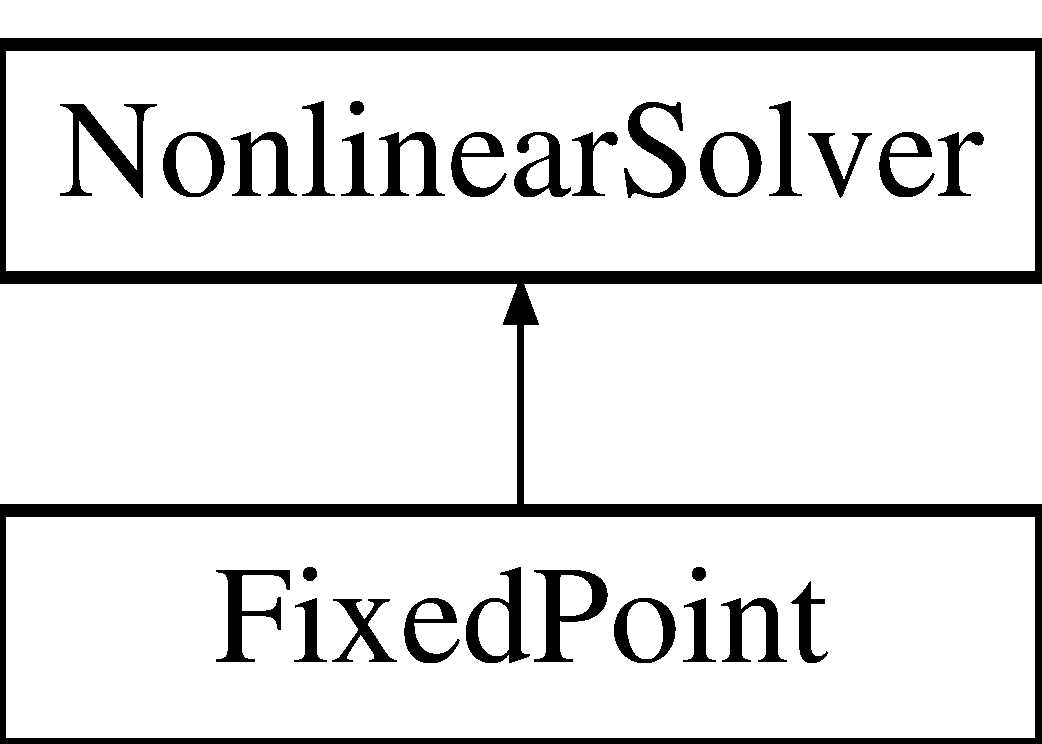
\includegraphics[height=2.000000cm]{class_fixed_point}
\end{center}
\end{figure}
\subsection*{Public Member Functions}
\begin{DoxyCompactItemize}
\item 
\hyperlink{class_fixed_point_aa5da7897eeeb9934b5f40b9b39b65464}{Fixed\+Point} (\hyperlink{class_expression}{Expression} \&equation, double initial, double tolerance, int max\+Iter, bool verbosity)
\item 
virtual \hyperlink{class_fixed_point_a489d5b95254cefb7248a3b2a9906464e}{$\sim$\+Fixed\+Point} ()\hypertarget{class_fixed_point_a489d5b95254cefb7248a3b2a9906464e}{}\label{class_fixed_point_a489d5b95254cefb7248a3b2a9906464e}

\begin{DoxyCompactList}\small\item\em A virtual destructor for the Fixed Point method. \end{DoxyCompactList}\item 
double \hyperlink{class_fixed_point_abc468159d11955a2a78a5278cf3339f6}{solve} ()
\end{DoxyCompactItemize}
\subsection*{Additional Inherited Members}


\subsection{Detailed Description}
\hyperlink{_fixed_point_8hpp_source}{Fixed\+Point.\+hpp}. 

A class constructing an object capable of solving nonlinear systems with the Fixed Point method. \begin{DoxyAuthor}{Author}
Jaquier, Michael \href{mailto:michael.jaquier@epfl.ch}{\tt michael.\+jaquier@epfl.\+ch} 

Lorkowski, Alexander \href{mailto:alexander.lorkowski@epfl.ch}{\tt alexander.\+lorkowski@epfl.\+ch} 
\end{DoxyAuthor}
\begin{DoxyVersion}{Version}
1.\+0 
\end{DoxyVersion}
\begin{DoxyDate}{Date}
10 December 2016 
\end{DoxyDate}
\begin{DoxyRemark}{Remarks}
Ecole Polytechnic Federal de Lausanne (E\+P\+FL) 

M\+A\+T\+H-\/458 Programming Concepts in Scientific Computing 
\end{DoxyRemark}


\subsection{Constructor \& Destructor Documentation}
\index{Fixed\+Point@{Fixed\+Point}!Fixed\+Point@{Fixed\+Point}}
\index{Fixed\+Point@{Fixed\+Point}!Fixed\+Point@{Fixed\+Point}}
\subsubsection[{\texorpdfstring{Fixed\+Point(\+Expression \&equation, double initial, double tolerance, int max\+Iter, bool verbosity)}{FixedPoint(Expression &equation, double initial, double tolerance, int maxIter, bool verbosity)}}]{\setlength{\rightskip}{0pt plus 5cm}Fixed\+Point\+::\+Fixed\+Point (
\begin{DoxyParamCaption}
\item[{{\bf Expression} \&}]{equation, }
\item[{double}]{initial, }
\item[{double}]{tolerance, }
\item[{int}]{max\+Iter, }
\item[{bool}]{verbosity}
\end{DoxyParamCaption}
)}\hypertarget{class_fixed_point_aa5da7897eeeb9934b5f40b9b39b65464}{}\label{class_fixed_point_aa5da7897eeeb9934b5f40b9b39b65464}
A constructor to instantiate variables for the Fixed Point method.


\begin{DoxyParams}{Parameters}
{\em equation} & A string that contains the mathematical expression for the class to evaluate. \\
\hline
{\em initial} & The initial guess of the solution to the equation. \\
\hline
{\em tolerance} & The tolerance value. The method stops once the residual errors fall below this value. \\
\hline
{\em max\+Iter} & The maximum number of iterations. The method stops once this number is reached. \\
\hline
{\em verbosity} & Set to true to print all intermediate and final results onto the console. \\
\hline
\end{DoxyParams}


\subsection{Member Function Documentation}
\index{Fixed\+Point@{Fixed\+Point}!solve@{solve}}
\index{solve@{solve}!Fixed\+Point@{Fixed\+Point}}
\subsubsection[{\texorpdfstring{solve()}{solve()}}]{\setlength{\rightskip}{0pt plus 5cm}double Fixed\+Point\+::solve (
\begin{DoxyParamCaption}
{}
\end{DoxyParamCaption}
)\hspace{0.3cm}{\ttfamily [virtual]}}\hypertarget{class_fixed_point_abc468159d11955a2a78a5278cf3339f6}{}\label{class_fixed_point_abc468159d11955a2a78a5278cf3339f6}
A function that returns the solution to the Fixed Point method.

\begin{DoxyReturn}{Returns}
The solution to the Fixed Point Method. 
\end{DoxyReturn}


Implements \hyperlink{class_nonlinear_solver_a72180277586bd7ec915cc4a806f62bb9}{Nonlinear\+Solver}.



The documentation for this class was generated from the following files\+:\begin{DoxyCompactItemize}
\item 
code/Fixed\+Point.\+hpp\item 
code/Fixed\+Point.\+cpp\end{DoxyCompactItemize}

\hypertarget{class_gauss}{}\section{Gauss Class Reference}
\label{class_gauss}\index{Gauss@{Gauss}}
Inheritance diagram for Gauss\+:\begin{figure}[H]
\begin{center}
\leavevmode
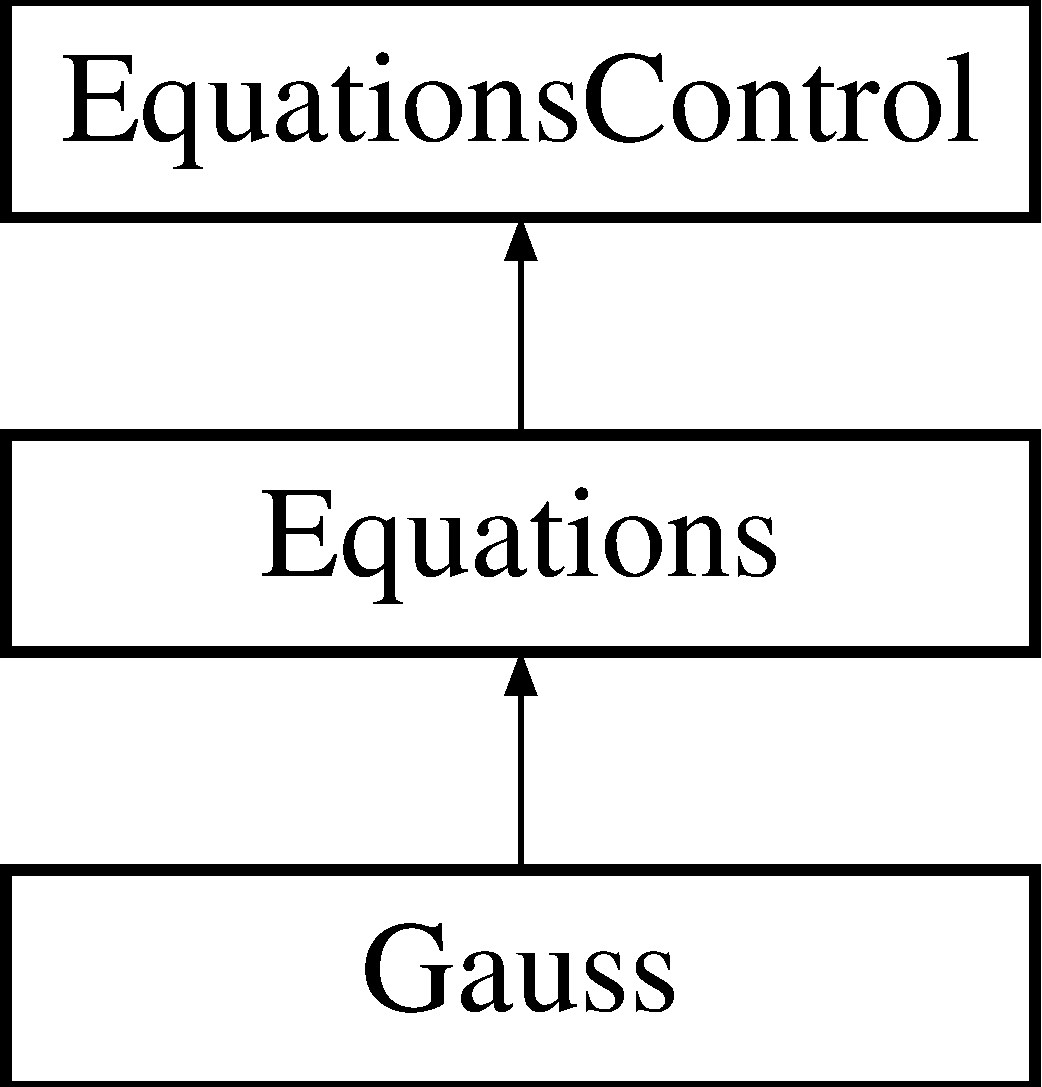
\includegraphics[height=3.000000cm]{class_gauss}
\end{center}
\end{figure}
\subsection*{Public Member Functions}
\begin{DoxyCompactItemize}
\end{DoxyCompactItemize}
\subsection*{Additional Inherited Members}


The documentation for this class was generated from the following files\+:\begin{DoxyCompactItemize}
\item 
code/Gauss.\+h\item 
code/Gauss.\+cpp\end{DoxyCompactItemize}

\hypertarget{class_helper}{}\section{Helper Class Reference}
\label{class_helper}\index{Helper@{Helper}}
\subsection*{Public Member Functions}
\begin{DoxyCompactItemize}
\item 
\hyperlink{class_helper_a900451b12f8e4c9ff5b17625446a245a}{Helper} (std\+::string name)
\item 
virtual \hyperlink{class_helper_ad714e92b4bc40bee681e0713503c9b27}{$\sim$\+Helper} ()\hypertarget{class_helper_ad714e92b4bc40bee681e0713503c9b27}{}\label{class_helper_ad714e92b4bc40bee681e0713503c9b27}

\begin{DoxyCompactList}\small\item\em A virtual destructor for the \hyperlink{class_newton}{Newton} method. \end{DoxyCompactList}\item 
void \hyperlink{class_helper_abbd7f229f433e467b7d8e1562c89e391}{show\+\_\+usage} ()\hypertarget{class_helper_abbd7f229f433e467b7d8e1562c89e391}{}\label{class_helper_abbd7f229f433e467b7d8e1562c89e391}

\begin{DoxyCompactList}\small\item\em A method that prints the usage screen onto the console. \end{DoxyCompactList}\item 
void \hyperlink{class_helper_aa560259807192d3feac483e88894bc64}{show\+\_\+methods} ()\hypertarget{class_helper_aa560259807192d3feac483e88894bc64}{}\label{class_helper_aa560259807192d3feac483e88894bc64}

\begin{DoxyCompactList}\small\item\em A method that prints implemented Nonlinear Solvers in the program. \end{DoxyCompactList}\end{DoxyCompactItemize}


\subsection{Constructor \& Destructor Documentation}
\index{Helper@{Helper}!Helper@{Helper}}
\index{Helper@{Helper}!Helper@{Helper}}
\subsubsection[{\texorpdfstring{Helper(std\+::string name)}{Helper(std::string name)}}]{\setlength{\rightskip}{0pt plus 5cm}Helper\+::\+Helper (
\begin{DoxyParamCaption}
\item[{std\+::string}]{name}
\end{DoxyParamCaption}
)}\hypertarget{class_helper_a900451b12f8e4c9ff5b17625446a245a}{}\label{class_helper_a900451b12f8e4c9ff5b17625446a245a}
A constructor to assign the program name to the helper class.


\begin{DoxyParams}{Parameters}
{\em name} & The name of the program. \\
\hline
\end{DoxyParams}


The documentation for this class was generated from the following files\+:\begin{DoxyCompactItemize}
\item 
code/Helper.\+hpp\item 
code/Helper.\+cpp\end{DoxyCompactItemize}

\hypertarget{class_initial_vector}{}\section{Initial\+Vector Class Reference}
\label{class_initial_vector}\index{Initial\+Vector@{Initial\+Vector}}
\subsection*{Public Member Functions}
\begin{DoxyCompactItemize}
\item 
\hyperlink{class_initial_vector_a4a8ad49cef57e0644dc18b937265b164}{Initial\+Vector} (std\+::string input)
\begin{DoxyCompactList}\small\item\em Constructor to generate the system of equations. \end{DoxyCompactList}\item 
\hyperlink{class_initial_vector_ace60dc8d6312008b9921b69c07ac2ca7}{Initial\+Vector} ()\hypertarget{class_initial_vector_ace60dc8d6312008b9921b69c07ac2ca7}{}\label{class_initial_vector_ace60dc8d6312008b9921b69c07ac2ca7}

\begin{DoxyCompactList}\small\item\em Constructor to generate the system of equations. \end{DoxyCompactList}\item 
virtual \hyperlink{class_initial_vector_aa18ee624f9f9bdd68e3d211cdccde055}{$\sim$\+Initial\+Vector} ()\hypertarget{class_initial_vector_aa18ee624f9f9bdd68e3d211cdccde055}{}\label{class_initial_vector_aa18ee624f9f9bdd68e3d211cdccde055}

\begin{DoxyCompactList}\small\item\em A virtual destructor for the Initial Vector class. \end{DoxyCompactList}\item 
std\+::vector$<$ double $>$ \hyperlink{class_initial_vector_af01341a5a32b28d6066632959566fecd}{get\+Values} ()\hypertarget{class_initial_vector_af01341a5a32b28d6066632959566fecd}{}\label{class_initial_vector_af01341a5a32b28d6066632959566fecd}

\begin{DoxyCompactList}\small\item\em Method to return the values contained in the vector. \end{DoxyCompactList}\item 
void \hyperlink{class_initial_vector_ae71fa73543bd36443fc19e3c87c7d205}{print} ()\hypertarget{class_initial_vector_ae71fa73543bd36443fc19e3c87c7d205}{}\label{class_initial_vector_ae71fa73543bd36443fc19e3c87c7d205}

\begin{DoxyCompactList}\small\item\em Method to print out the equations. \end{DoxyCompactList}\item 
double \hyperlink{class_initial_vector_a8f822bce7ca795f2be49862c87c5a3e2}{get\+Value} (int i)
\begin{DoxyCompactList}\small\item\em Method to return an individual equation from the system matrix. \end{DoxyCompactList}\end{DoxyCompactItemize}


\subsection{Constructor \& Destructor Documentation}
\index{Initial\+Vector@{Initial\+Vector}!Initial\+Vector@{Initial\+Vector}}
\index{Initial\+Vector@{Initial\+Vector}!Initial\+Vector@{Initial\+Vector}}
\subsubsection[{\texorpdfstring{Initial\+Vector(std\+::string input)}{InitialVector(std::string input)}}]{\setlength{\rightskip}{0pt plus 5cm}Initial\+Vector\+::\+Initial\+Vector (
\begin{DoxyParamCaption}
\item[{std\+::string}]{input}
\end{DoxyParamCaption}
)}\hypertarget{class_initial_vector_a4a8ad49cef57e0644dc18b937265b164}{}\label{class_initial_vector_a4a8ad49cef57e0644dc18b937265b164}


Constructor to generate the system of equations. 


\begin{DoxyParams}{Parameters}
{\em input} & -\/ The file name containing equations. \\
\hline
\end{DoxyParams}


\subsection{Member Function Documentation}
\index{Initial\+Vector@{Initial\+Vector}!get\+Value@{get\+Value}}
\index{get\+Value@{get\+Value}!Initial\+Vector@{Initial\+Vector}}
\subsubsection[{\texorpdfstring{get\+Value(int i)}{getValue(int i)}}]{\setlength{\rightskip}{0pt plus 5cm}double Initial\+Vector\+::get\+Value (
\begin{DoxyParamCaption}
\item[{int}]{i}
\end{DoxyParamCaption}
)}\hypertarget{class_initial_vector_a8f822bce7ca795f2be49862c87c5a3e2}{}\label{class_initial_vector_a8f822bce7ca795f2be49862c87c5a3e2}


Method to return an individual equation from the system matrix. 


\begin{DoxyParams}{Parameters}
{\em i} & The index of the value to be returned. \\
\hline
\end{DoxyParams}
\begin{DoxyReturn}{Returns}
Returns a \hyperlink{class_expression}{Expression} which contains a single equation. 
\end{DoxyReturn}


The documentation for this class was generated from the following files\+:\begin{DoxyCompactItemize}
\item 
code/Initial\+Vector.\+hpp\item 
code/Initial\+Vector.\+cpp\end{DoxyCompactItemize}

\hypertarget{class_newton}{}\section{Newton Class Reference}
\label{class_newton}\index{Newton@{Newton}}


\hyperlink{_newton_8hpp_source}{Newton.\+hpp}.  




{\ttfamily \#include $<$Newton.\+hpp$>$}

Inheritance diagram for Newton\+:\begin{figure}[H]
\begin{center}
\leavevmode
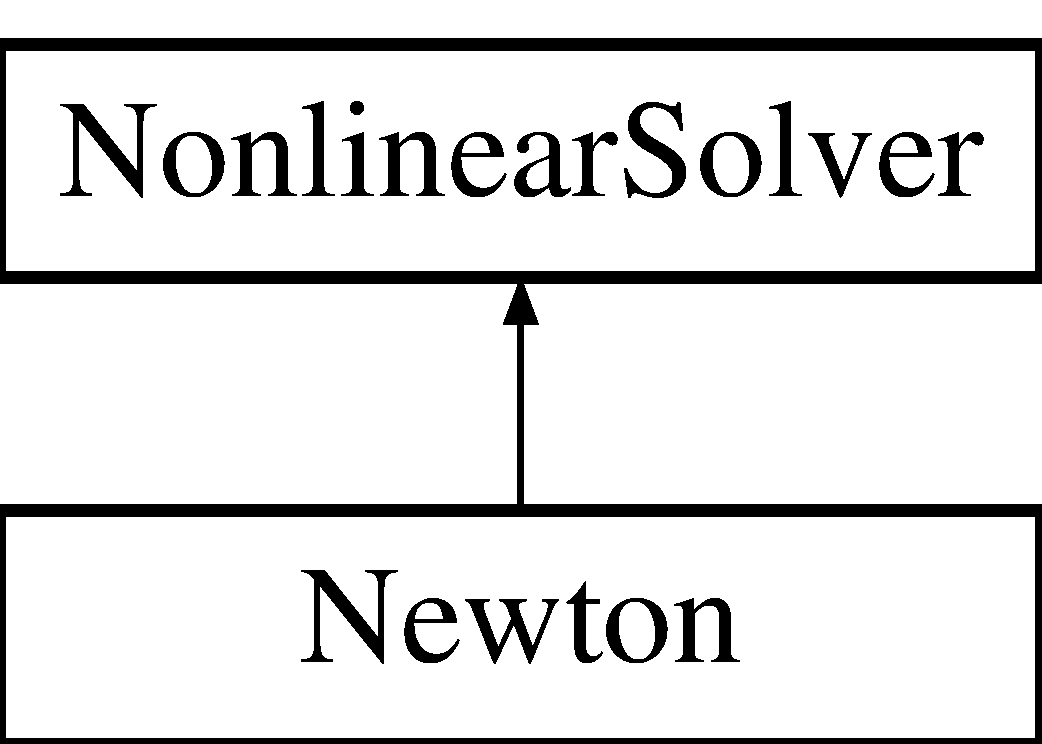
\includegraphics[height=2.000000cm]{class_newton}
\end{center}
\end{figure}
\subsection*{Public Member Functions}
\begin{DoxyCompactItemize}
\item 
\hyperlink{class_newton_ac64453229e5ac9ceee846bbefbb3d3e2}{Newton} (\hyperlink{class_expression}{Expression} \&equation, \hyperlink{class_expression}{Expression} \&derivative, double initial, double tolerance, int max\+Iter, bool verbosity)
\item 
\hyperlink{class_newton_a076a4ed0ada157318fda266cbdc78b08}{Newton} (\hyperlink{class_expression}{Expression} \&equation, \hyperlink{class_expression}{Expression} \&derivative, double initial, double tolerance, int max\+Iter, bool verbosity, int modifier)
\item 
virtual \hyperlink{class_newton_a12782031a0e3dc0806ee5e4774d8ab35}{$\sim$\+Newton} ()\hypertarget{class_newton_a12782031a0e3dc0806ee5e4774d8ab35}{}\label{class_newton_a12782031a0e3dc0806ee5e4774d8ab35}

\begin{DoxyCompactList}\small\item\em A virtual destructor for the \hyperlink{class_newton}{Newton} method. \end{DoxyCompactList}\item 
double \hyperlink{class_newton_a09981094747d53116cf7a4a5194d8787}{solve} ()
\end{DoxyCompactItemize}
\subsection*{Additional Inherited Members}


\subsection{Detailed Description}
\hyperlink{_newton_8hpp_source}{Newton.\+hpp}. 

A class constructing an object capable of solving nonlinear systems with the \hyperlink{class_newton}{Newton} method. \begin{DoxyAuthor}{Author}
Jaquier, Michael \href{mailto:michael.jaquier@epfl.ch}{\tt michael.\+jaquier@epfl.\+ch} 

Lorkowski, Alexander \href{mailto:alexander.lorkowski@epfl.ch}{\tt alexander.\+lorkowski@epfl.\+ch} 
\end{DoxyAuthor}
\begin{DoxyVersion}{Version}
1.\+0 
\end{DoxyVersion}
\begin{DoxyDate}{Date}
10 December 2016 
\end{DoxyDate}
\begin{DoxyRemark}{Remarks}
Ecole Polytechnic Federal de Lausanne (E\+P\+FL) 

M\+A\+T\+H-\/458 Programming Concepts in Scientific Computing 
\end{DoxyRemark}


\subsection{Constructor \& Destructor Documentation}
\index{Newton@{Newton}!Newton@{Newton}}
\index{Newton@{Newton}!Newton@{Newton}}
\subsubsection[{\texorpdfstring{Newton(\+Expression \&equation, Expression \&derivative, double initial, double tolerance, int max\+Iter, bool verbosity)}{Newton(Expression &equation, Expression &derivative, double initial, double tolerance, int maxIter, bool verbosity)}}]{\setlength{\rightskip}{0pt plus 5cm}Newton\+::\+Newton (
\begin{DoxyParamCaption}
\item[{{\bf Expression} \&}]{equation, }
\item[{{\bf Expression} \&}]{derivative, }
\item[{double}]{initial, }
\item[{double}]{tolerance, }
\item[{int}]{max\+Iter, }
\item[{bool}]{verbosity}
\end{DoxyParamCaption}
)}\hypertarget{class_newton_ac64453229e5ac9ceee846bbefbb3d3e2}{}\label{class_newton_ac64453229e5ac9ceee846bbefbb3d3e2}
A constructor to instantiate variables for the Newtwon method.


\begin{DoxyParams}{Parameters}
{\em equation} & A string that contains the mathematical expression for the class to evaluate. \\
\hline
{\em derivative} & A string that contains the derivative of the expression for the class to evaluate. \\
\hline
{\em initial} & The initial guess of the solution to the equation. \\
\hline
{\em tolerance} & The tolerance value. The method stops once the residual errors fall below this value. \\
\hline
{\em max\+Iter} & The maximum number of iterations. The method stops once this number is reached. \\
\hline
{\em verbosity} & Set to true to print all intermediate and final results onto the console. \\
\hline
\end{DoxyParams}
\index{Newton@{Newton}!Newton@{Newton}}
\index{Newton@{Newton}!Newton@{Newton}}
\subsubsection[{\texorpdfstring{Newton(\+Expression \&equation, Expression \&derivative, double initial, double tolerance, int max\+Iter, bool verbosity, int modifier)}{Newton(Expression &equation, Expression &derivative, double initial, double tolerance, int maxIter, bool verbosity, int modifier)}}]{\setlength{\rightskip}{0pt plus 5cm}Newton\+::\+Newton (
\begin{DoxyParamCaption}
\item[{{\bf Expression} \&}]{equation, }
\item[{{\bf Expression} \&}]{derivative, }
\item[{double}]{initial, }
\item[{double}]{tolerance, }
\item[{int}]{max\+Iter, }
\item[{bool}]{verbosity, }
\item[{int}]{modifier}
\end{DoxyParamCaption}
)}\hypertarget{class_newton_a076a4ed0ada157318fda266cbdc78b08}{}\label{class_newton_a076a4ed0ada157318fda266cbdc78b08}
A constructor to instantiate variables for the modified Newtwon method.


\begin{DoxyParams}{Parameters}
{\em equation} & A string that contains the mathematical expression for the class to evaluate. \\
\hline
{\em derivative} & A string that contains the derivative of the expression for the class to evaluate. \\
\hline
{\em initial} & The initial guess of the solution to the equation. \\
\hline
{\em tolerance} & The tolerance value. The method stops once the residual errors fall below this value. \\
\hline
{\em max\+Iter} & The maximum number of iterations. The method stops once this number is reached. \\
\hline
{\em verbosity} & Set to true to print all intermediate and final results onto the console. \\
\hline
{\em modifier} & The integer value for the modified \hyperlink{class_newton}{Newton} method. \\
\hline
\end{DoxyParams}


\subsection{Member Function Documentation}
\index{Newton@{Newton}!solve@{solve}}
\index{solve@{solve}!Newton@{Newton}}
\subsubsection[{\texorpdfstring{solve()}{solve()}}]{\setlength{\rightskip}{0pt plus 5cm}double Newton\+::solve (
\begin{DoxyParamCaption}
{}
\end{DoxyParamCaption}
)\hspace{0.3cm}{\ttfamily [virtual]}}\hypertarget{class_newton_a09981094747d53116cf7a4a5194d8787}{}\label{class_newton_a09981094747d53116cf7a4a5194d8787}
A function when called returns the solution to the \hyperlink{class_newton}{Newton} Method/\+Modified \hyperlink{class_newton}{Newton} Method.

\begin{DoxyReturn}{Returns}
The solution to the \hyperlink{class_newton}{Newton} Method/\+Modified \hyperlink{class_newton}{Newton} Method. 
\end{DoxyReturn}


Implements \hyperlink{class_nonlinear_solver_a72180277586bd7ec915cc4a806f62bb9}{Nonlinear\+Solver}.



The documentation for this class was generated from the following files\+:\begin{DoxyCompactItemize}
\item 
code/Newton.\+hpp\item 
code/Newton.\+cpp\end{DoxyCompactItemize}

\hypertarget{class_newton_system}{}\section{Newton\+System Class Reference}
\label{class_newton_system}\index{Newton\+System@{Newton\+System}}
Inheritance diagram for Newton\+System\+:\begin{figure}[H]
\begin{center}
\leavevmode
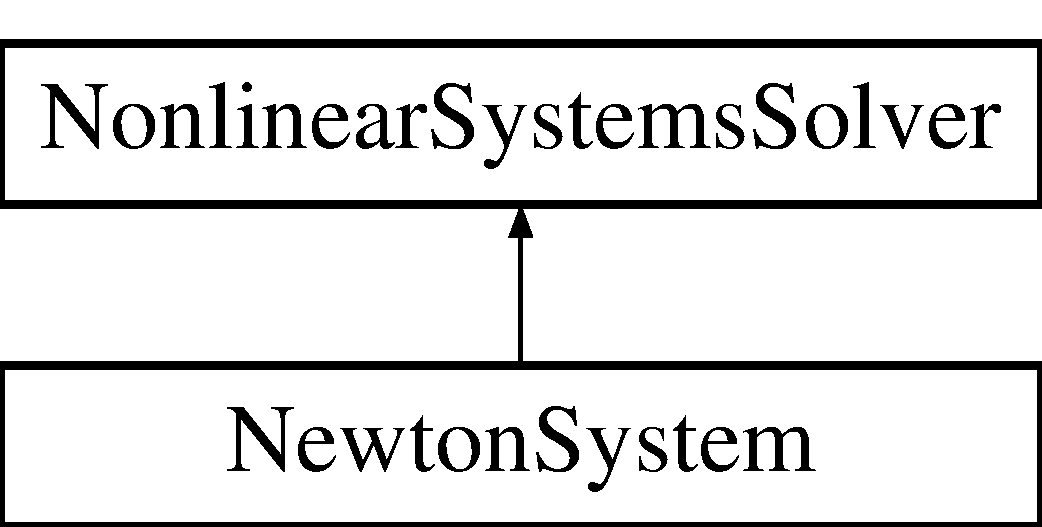
\includegraphics[height=2.000000cm]{class_newton_system}
\end{center}
\end{figure}
\subsection*{Public Member Functions}
\begin{DoxyCompactItemize}
\item 
\hyperlink{class_newton_system_a0b9c529d0f7357b70bfb67edad9627e6}{Newton\+System} (\hyperlink{class_expression_system}{Expression\+System} \&\hyperlink{class_nonlinear_systems_solver_ad58bb6449941acd3f88bc5647b4c8068}{system}, \hyperlink{class_expression_system}{Expression\+System} \&jacobian, std\+::vector$<$ double $>$ \&initial, double tolerance, int max\+Iter, bool verbosity, int mod)
\begin{DoxyCompactList}\small\item\em \hyperlink{class_newton}{Newton} -\/ solver for a system of equations. \end{DoxyCompactList}\item 
virtual \hyperlink{class_newton_system_aef07a5a77f0a12fb18493239e38c816b}{$\sim$\+Newton\+System} ()\hypertarget{class_newton_system_aef07a5a77f0a12fb18493239e38c816b}{}\label{class_newton_system_aef07a5a77f0a12fb18493239e38c816b}

\begin{DoxyCompactList}\small\item\em A virtual destructor for the \hyperlink{class_newton}{Newton} System method. \end{DoxyCompactList}\item 
std\+::vector$<$ double $>$ \hyperlink{class_newton_system_ad75a80fbdf3598310c5e9497a7aad5d7}{solve} ()
\begin{DoxyCompactList}\small\item\em solves the system of equations uses recursive calls to \hyperlink{class_expression}{Expression} class \end{DoxyCompactList}\item 
void \hyperlink{class_newton_system_a06277d1bff35436d6ef260a9ecb4117c}{apply\+Modifier} (std\+::vector$<$ double $>$ \&dxyz)
\begin{DoxyCompactList}\small\item\em Applies the newton modification to each element. \end{DoxyCompactList}\end{DoxyCompactItemize}
\subsection*{Additional Inherited Members}


\subsection{Constructor \& Destructor Documentation}
\index{Newton\+System@{Newton\+System}!Newton\+System@{Newton\+System}}
\index{Newton\+System@{Newton\+System}!Newton\+System@{Newton\+System}}
\subsubsection[{\texorpdfstring{Newton\+System(\+Expression\+System \&system, Expression\+System \&jacobian, std\+::vector$<$ double $>$ \&initial, double tolerance, int max\+Iter, bool verbosity, int mod)}{NewtonSystem(ExpressionSystem &system, ExpressionSystem &jacobian, std::vector< double > &initial, double tolerance, int maxIter, bool verbosity, int mod)}}]{\setlength{\rightskip}{0pt plus 5cm}Newton\+System\+::\+Newton\+System (
\begin{DoxyParamCaption}
\item[{{\bf Expression\+System} \&}]{system, }
\item[{{\bf Expression\+System} \&}]{jacobian, }
\item[{std\+::vector$<$ double $>$ \&}]{initial, }
\item[{double}]{tolerance, }
\item[{int}]{max\+Iter, }
\item[{bool}]{verbosity, }
\item[{int}]{mod}
\end{DoxyParamCaption}
)}\hypertarget{class_newton_system_a0b9c529d0f7357b70bfb67edad9627e6}{}\label{class_newton_system_a0b9c529d0f7357b70bfb67edad9627e6}


\hyperlink{class_newton}{Newton} -\/ solver for a system of equations. 


\begin{DoxyParams}{Parameters}
{\em system} & -\/ The system of equations \\
\hline
{\em jacobian} & -\/ The jacobian of the system \\
\hline
{\em initial} & -\/ Initial guess provided by user \\
\hline
{\em tolerance} & -\/ The numeric tolerance allowed for the solution \\
\hline
{\em max\+Iter} & -\/ The maximum iterations allowed for a solution \\
\hline
{\em verbosity} & -\/ Print intermediate steps \\
\hline
{\em mod} & -\/ Set the modifying power of the Steps. \\
\hline
\end{DoxyParams}


\subsection{Member Function Documentation}
\index{Newton\+System@{Newton\+System}!apply\+Modifier@{apply\+Modifier}}
\index{apply\+Modifier@{apply\+Modifier}!Newton\+System@{Newton\+System}}
\subsubsection[{\texorpdfstring{apply\+Modifier(std\+::vector$<$ double $>$ \&dxyz)}{applyModifier(std::vector< double > &dxyz)}}]{\setlength{\rightskip}{0pt plus 5cm}void Newton\+System\+::apply\+Modifier (
\begin{DoxyParamCaption}
\item[{std\+::vector$<$ double $>$ \&}]{dxyz}
\end{DoxyParamCaption}
)}\hypertarget{class_newton_system_a06277d1bff35436d6ef260a9ecb4117c}{}\label{class_newton_system_a06277d1bff35436d6ef260a9ecb4117c}


Applies the newton modification to each element. 


\begin{DoxyParams}{Parameters}
{\em dxyz} & \\
\hline
\end{DoxyParams}
\index{Newton\+System@{Newton\+System}!solve@{solve}}
\index{solve@{solve}!Newton\+System@{Newton\+System}}
\subsubsection[{\texorpdfstring{solve()}{solve()}}]{\setlength{\rightskip}{0pt plus 5cm}std\+::vector$<$ double $>$ Newton\+System\+::solve (
\begin{DoxyParamCaption}
{}
\end{DoxyParamCaption}
)\hspace{0.3cm}{\ttfamily [virtual]}}\hypertarget{class_newton_system_ad75a80fbdf3598310c5e9497a7aad5d7}{}\label{class_newton_system_ad75a80fbdf3598310c5e9497a7aad5d7}


solves the system of equations uses recursive calls to \hyperlink{class_expression}{Expression} class 

\begin{DoxyReturn}{Returns}
returns a vector of solutions 
\end{DoxyReturn}


Implements \hyperlink{class_nonlinear_systems_solver_a9067a4fa26bce4b2aa359cfccd93c84f}{Nonlinear\+Systems\+Solver}.



The documentation for this class was generated from the following files\+:\begin{DoxyCompactItemize}
\item 
code/Newton\+System.\+hpp\item 
code/Newton\+System.\+cpp\end{DoxyCompactItemize}

\hypertarget{class_nonlinear_solver}{}\section{Nonlinear\+Solver Class Reference}
\label{class_nonlinear_solver}\index{Nonlinear\+Solver@{Nonlinear\+Solver}}


\hyperlink{_nonlinear_solver_8hpp_source}{Nonlinear\+Solver.\+hpp}.  




{\ttfamily \#include $<$Nonlinear\+Solver.\+hpp$>$}

Inheritance diagram for Nonlinear\+Solver\+:\begin{figure}[H]
\begin{center}
\leavevmode
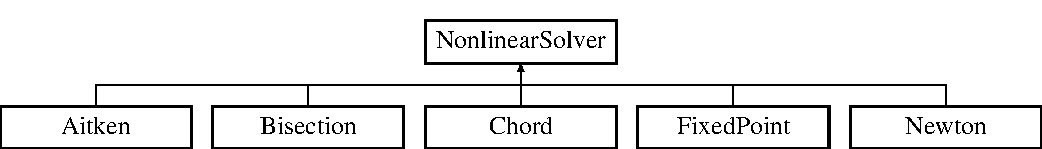
\includegraphics[height=2.000000cm]{class_nonlinear_solver}
\end{center}
\end{figure}
\subsection*{Public Member Functions}
\begin{DoxyCompactItemize}
\item 
\hyperlink{class_nonlinear_solver_af47ece967a93e6cfaf5b46bff22f6279}{Nonlinear\+Solver} (\hyperlink{class_expression}{Expression} \&equation, double initial, double tolerance, int max\+Iter, bool verbosity)
\item 
virtual \hyperlink{class_nonlinear_solver_ad29eabca357434c5e40764a80ee8482f}{$\sim$\+Nonlinear\+Solver} ()\hypertarget{class_nonlinear_solver_ad29eabca357434c5e40764a80ee8482f}{}\label{class_nonlinear_solver_ad29eabca357434c5e40764a80ee8482f}

\begin{DoxyCompactList}\small\item\em A virtual destructor for the family of nonlinear solvers. \end{DoxyCompactList}\item 
virtual double \hyperlink{class_nonlinear_solver_a72180277586bd7ec915cc4a806f62bb9}{solve} ()=0\hypertarget{class_nonlinear_solver_a72180277586bd7ec915cc4a806f62bb9}{}\label{class_nonlinear_solver_a72180277586bd7ec915cc4a806f62bb9}

\begin{DoxyCompactList}\small\item\em A pure virtual solver method for the family of nonlinear solvers. \end{DoxyCompactList}\item 
void \hyperlink{class_nonlinear_solver_ac27b68fb52e995ee5204b255460a3e13}{print\+Verbose} (int i, double \&x)
\end{DoxyCompactItemize}
\subsection*{Protected Attributes}
\begin{DoxyCompactItemize}
\item 
\hyperlink{class_expression}{Expression} \hyperlink{class_nonlinear_solver_aad588fc96d07cf310a13ae11b51ce550}{eq}\hypertarget{class_nonlinear_solver_aad588fc96d07cf310a13ae11b51ce550}{}\label{class_nonlinear_solver_aad588fc96d07cf310a13ae11b51ce550}

\begin{DoxyCompactList}\small\item\em An object of the \hyperlink{class_expression}{Expression} class holding the strings representing mathematical expressions. \end{DoxyCompactList}\item 
double \hyperlink{class_nonlinear_solver_a0af503b5f79fd74a61b1ba8c956e9a06}{x0}\hypertarget{class_nonlinear_solver_a0af503b5f79fd74a61b1ba8c956e9a06}{}\label{class_nonlinear_solver_a0af503b5f79fd74a61b1ba8c956e9a06}

\begin{DoxyCompactList}\small\item\em A doubles representing the initial guess of the solution to the equation. \end{DoxyCompactList}\item 
double \hyperlink{class_nonlinear_solver_a8fa50d85cb58f69da6cddf52a2b950af}{tol}\hypertarget{class_nonlinear_solver_a8fa50d85cb58f69da6cddf52a2b950af}{}\label{class_nonlinear_solver_a8fa50d85cb58f69da6cddf52a2b950af}

\begin{DoxyCompactList}\small\item\em The tolerance value. The method stops once the residual errors fall below this value. \end{DoxyCompactList}\item 
int \hyperlink{class_nonlinear_solver_accd5129e5d683f9d8187bd9d4d13b023}{n\+Max}\hypertarget{class_nonlinear_solver_accd5129e5d683f9d8187bd9d4d13b023}{}\label{class_nonlinear_solver_accd5129e5d683f9d8187bd9d4d13b023}

\begin{DoxyCompactList}\small\item\em The maximum number of iterations. The method stops once this number is reached. \end{DoxyCompactList}\item 
bool \hyperlink{class_nonlinear_solver_a81db23a90d44eeea9b9ec57d8ea94155}{verbose}\hypertarget{class_nonlinear_solver_a81db23a90d44eeea9b9ec57d8ea94155}{}\label{class_nonlinear_solver_a81db23a90d44eeea9b9ec57d8ea94155}

\begin{DoxyCompactList}\small\item\em Set to true to print all intermediate and final results onto the console. \end{DoxyCompactList}\end{DoxyCompactItemize}


\subsection{Detailed Description}
\hyperlink{_nonlinear_solver_8hpp_source}{Nonlinear\+Solver.\+hpp}. 

An abstract class for the family of nonlinear solvers. \begin{DoxyAuthor}{Author}
Jaquier, Michael \href{mailto:michael.jaquier@epfl.ch}{\tt michael.\+jaquier@epfl.\+ch} 

Lorkowski, Alexander \href{mailto:alexander.lorkowski@epfl.ch}{\tt alexander.\+lorkowski@epfl.\+ch} 
\end{DoxyAuthor}
\begin{DoxyVersion}{Version}
1.\+0 
\end{DoxyVersion}
\begin{DoxyDate}{Date}
10 December 2016 
\end{DoxyDate}
\begin{DoxyRemark}{Remarks}
Ecole Polytechnic Federal de Lausanne (E\+P\+FL) 

M\+A\+T\+H-\/458 Programming Concepts in Scientific Computing 
\end{DoxyRemark}


\subsection{Constructor \& Destructor Documentation}
\index{Nonlinear\+Solver@{Nonlinear\+Solver}!Nonlinear\+Solver@{Nonlinear\+Solver}}
\index{Nonlinear\+Solver@{Nonlinear\+Solver}!Nonlinear\+Solver@{Nonlinear\+Solver}}
\subsubsection[{\texorpdfstring{Nonlinear\+Solver(\+Expression \&equation, double initial, double tolerance, int max\+Iter, bool verbosity)}{NonlinearSolver(Expression &equation, double initial, double tolerance, int maxIter, bool verbosity)}}]{\setlength{\rightskip}{0pt plus 5cm}Nonlinear\+Solver\+::\+Nonlinear\+Solver (
\begin{DoxyParamCaption}
\item[{{\bf Expression} \&}]{equation, }
\item[{double}]{initial, }
\item[{double}]{tolerance, }
\item[{int}]{max\+Iter, }
\item[{bool}]{verbosity}
\end{DoxyParamCaption}
)}\hypertarget{class_nonlinear_solver_af47ece967a93e6cfaf5b46bff22f6279}{}\label{class_nonlinear_solver_af47ece967a93e6cfaf5b46bff22f6279}
A contructor to instantiate common variables to the family of nonlinear solvers.


\begin{DoxyParams}{Parameters}
{\em equation} & An object of the \hyperlink{class_expression}{Expression} class that contains the mathematical expression for the class to evaluate. \\
\hline
{\em initial} & The initial guess of the solution to the equation. \\
\hline
{\em tolerance} & The tolerance value. The method stops once the residual errors fall below this value. \\
\hline
{\em max\+Iter} & The maximum number of iterations. The method stops once this number is reached. \\
\hline
{\em verbosity} & Set to true to print all intermediate and final results onto the console. \\
\hline
\end{DoxyParams}


\subsection{Member Function Documentation}
\index{Nonlinear\+Solver@{Nonlinear\+Solver}!print\+Verbose@{print\+Verbose}}
\index{print\+Verbose@{print\+Verbose}!Nonlinear\+Solver@{Nonlinear\+Solver}}
\subsubsection[{\texorpdfstring{print\+Verbose(int i, double \&x)}{printVerbose(int i, double &x)}}]{\setlength{\rightskip}{0pt plus 5cm}void Nonlinear\+Solver\+::print\+Verbose (
\begin{DoxyParamCaption}
\item[{int}]{i, }
\item[{double \&}]{x}
\end{DoxyParamCaption}
)}\hypertarget{class_nonlinear_solver_ac27b68fb52e995ee5204b255460a3e13}{}\label{class_nonlinear_solver_ac27b68fb52e995ee5204b255460a3e13}
A function that takes a constant integer and a vector argument and prints to the console.


\begin{DoxyParams}{Parameters}
{\em i} & The current index or iteration to print out to the console. \\
\hline
{\em x} & The current solution of the nonlinear problem. \\
\hline
\end{DoxyParams}


The documentation for this class was generated from the following files\+:\begin{DoxyCompactItemize}
\item 
code/Nonlinear\+Solver.\+hpp\item 
code/Nonlinear\+Solver.\+cpp\end{DoxyCompactItemize}

\hypertarget{class_nonlinear_systems_solver}{}\section{Nonlinear\+Systems\+Solver Class Reference}
\label{class_nonlinear_systems_solver}\index{Nonlinear\+Systems\+Solver@{Nonlinear\+Systems\+Solver}}


\hyperlink{_nonlinear_systems_solver_8hpp_source}{Nonlinear\+Systems\+Solver.\+hpp}.  




{\ttfamily \#include $<$Nonlinear\+Systems\+Solver.\+hpp$>$}

Inheritance diagram for Nonlinear\+Systems\+Solver\+:\begin{figure}[H]
\begin{center}
\leavevmode
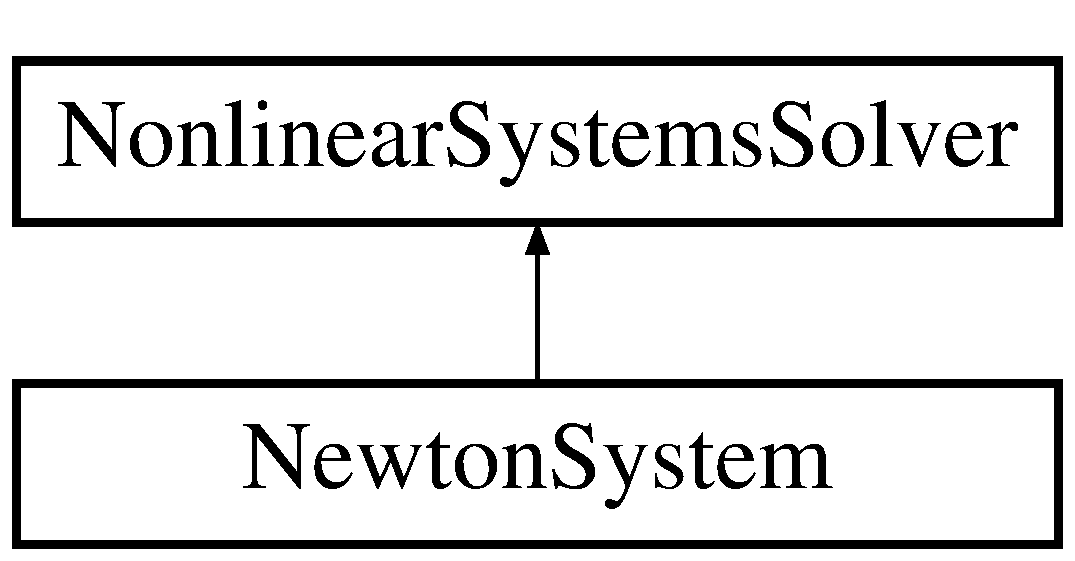
\includegraphics[height=2.000000cm]{class_nonlinear_systems_solver}
\end{center}
\end{figure}
\subsection*{Public Member Functions}
\begin{DoxyCompactItemize}
\item 
\hyperlink{class_nonlinear_systems_solver_a39b82503490941b7972fde0cfbd28ca0}{Nonlinear\+Systems\+Solver} (\hyperlink{class_expression_system}{Expression\+System} \&sys, std\+::vector$<$ double $>$ \&initial, double tolerance, int max\+Iter, bool verbosity)
\item 
virtual \hyperlink{class_nonlinear_systems_solver_a7a2bc7ca31192bf419d595abd887bd11}{$\sim$\+Nonlinear\+Systems\+Solver} ()\hypertarget{class_nonlinear_systems_solver_a7a2bc7ca31192bf419d595abd887bd11}{}\label{class_nonlinear_systems_solver_a7a2bc7ca31192bf419d595abd887bd11}

\begin{DoxyCompactList}\small\item\em A virtual destructor for the family of nonlinear solvers. \end{DoxyCompactList}\item 
virtual std\+::vector$<$ double $>$ \hyperlink{class_nonlinear_systems_solver_a9067a4fa26bce4b2aa359cfccd93c84f}{solve} ()=0\hypertarget{class_nonlinear_systems_solver_a9067a4fa26bce4b2aa359cfccd93c84f}{}\label{class_nonlinear_systems_solver_a9067a4fa26bce4b2aa359cfccd93c84f}

\begin{DoxyCompactList}\small\item\em A pure virtual solver method for the family of nonlinear solvers. \end{DoxyCompactList}\item 
void \hyperlink{class_nonlinear_systems_solver_ad071f60a5c0e9d714450ff71942891f4}{print\+Verbose} (int i, std\+::vector$<$ double $>$ \&v)
\end{DoxyCompactItemize}
\subsection*{Protected Attributes}
\begin{DoxyCompactItemize}
\item 
\hyperlink{class_expression_system}{Expression\+System} \hyperlink{class_nonlinear_systems_solver_ad58bb6449941acd3f88bc5647b4c8068}{system}\hypertarget{class_nonlinear_systems_solver_ad58bb6449941acd3f88bc5647b4c8068}{}\label{class_nonlinear_systems_solver_ad58bb6449941acd3f88bc5647b4c8068}

\begin{DoxyCompactList}\small\item\em A standard vector holding the strings representing mathematical expressions. \end{DoxyCompactList}\item 
std\+::vector$<$ double $>$ \hyperlink{class_nonlinear_systems_solver_a9733d9d1f170044dbefe980945070ba3}{v0}\hypertarget{class_nonlinear_systems_solver_a9733d9d1f170044dbefe980945070ba3}{}\label{class_nonlinear_systems_solver_a9733d9d1f170044dbefe980945070ba3}

\begin{DoxyCompactList}\small\item\em A standard vector holding the doubles representing the initial guess of the solution to the equation. \end{DoxyCompactList}\item 
double \hyperlink{class_nonlinear_systems_solver_a526132d9a95f69bd0e84682f61b5e732}{tol}\hypertarget{class_nonlinear_systems_solver_a526132d9a95f69bd0e84682f61b5e732}{}\label{class_nonlinear_systems_solver_a526132d9a95f69bd0e84682f61b5e732}

\begin{DoxyCompactList}\small\item\em The tolerance value. The method stops once the residual errors fall below this value. \end{DoxyCompactList}\item 
int \hyperlink{class_nonlinear_systems_solver_aa0075f162a80bd76fb2b05947f880eb3}{n\+Max}\hypertarget{class_nonlinear_systems_solver_aa0075f162a80bd76fb2b05947f880eb3}{}\label{class_nonlinear_systems_solver_aa0075f162a80bd76fb2b05947f880eb3}

\begin{DoxyCompactList}\small\item\em The maximum number of iterations. The method stops once this number is reached. \end{DoxyCompactList}\item 
bool \hyperlink{class_nonlinear_systems_solver_a3080b2ab66741d474b5a9a4f2244b5a7}{verbose}\hypertarget{class_nonlinear_systems_solver_a3080b2ab66741d474b5a9a4f2244b5a7}{}\label{class_nonlinear_systems_solver_a3080b2ab66741d474b5a9a4f2244b5a7}

\begin{DoxyCompactList}\small\item\em Set to true to print all intermediate and final results onto the console. \end{DoxyCompactList}\end{DoxyCompactItemize}


\subsection{Detailed Description}
\hyperlink{_nonlinear_systems_solver_8hpp_source}{Nonlinear\+Systems\+Solver.\+hpp}. 

An abstract class for the family of solvers of nonlinear systems. \begin{DoxyAuthor}{Author}
Jaquier, Michael \href{mailto:michael.jaquier@epfl.ch}{\tt michael.\+jaquier@epfl.\+ch} 

Lorkowski, Alexander \href{mailto:alexander.lorkowski@epfl.ch}{\tt alexander.\+lorkowski@epfl.\+ch} 
\end{DoxyAuthor}
\begin{DoxyVersion}{Version}
1.\+0 
\end{DoxyVersion}
\begin{DoxyDate}{Date}
10 December 2016 
\end{DoxyDate}
\begin{DoxyRemark}{Remarks}
Ecole Polytechnic Federal de Lausanne (E\+P\+FL) 

M\+A\+T\+H-\/458 Programming Concepts in Scientific Computing 
\end{DoxyRemark}


\subsection{Constructor \& Destructor Documentation}
\index{Nonlinear\+Systems\+Solver@{Nonlinear\+Systems\+Solver}!Nonlinear\+Systems\+Solver@{Nonlinear\+Systems\+Solver}}
\index{Nonlinear\+Systems\+Solver@{Nonlinear\+Systems\+Solver}!Nonlinear\+Systems\+Solver@{Nonlinear\+Systems\+Solver}}
\subsubsection[{\texorpdfstring{Nonlinear\+Systems\+Solver(\+Expression\+System \&sys, std\+::vector$<$ double $>$ \&initial, double tolerance, int max\+Iter, bool verbosity)}{NonlinearSystemsSolver(ExpressionSystem &sys, std::vector< double > &initial, double tolerance, int maxIter, bool verbosity)}}]{\setlength{\rightskip}{0pt plus 5cm}Nonlinear\+Systems\+Solver\+::\+Nonlinear\+Systems\+Solver (
\begin{DoxyParamCaption}
\item[{{\bf Expression\+System} \&}]{sys, }
\item[{std\+::vector$<$ double $>$ \&}]{initial, }
\item[{double}]{tolerance, }
\item[{int}]{max\+Iter, }
\item[{bool}]{verbosity}
\end{DoxyParamCaption}
)}\hypertarget{class_nonlinear_systems_solver_a39b82503490941b7972fde0cfbd28ca0}{}\label{class_nonlinear_systems_solver_a39b82503490941b7972fde0cfbd28ca0}
A contructor to instantiate common variables to the family of nonlinear solvers.


\begin{DoxyParams}{Parameters}
{\em sys} & An \hyperlink{class_expression_system}{Expression\+System} object containing the system of equations. \\
\hline
{\em initial} & The initial guess of the solution to the equation. \\
\hline
{\em tolerance} & The tolerance value. The method stops once the residual errors fall below this value. \\
\hline
{\em max\+Iter} & The maximum number of iterations. The method stops once this number is reached. \\
\hline
{\em verbosity} & Set to true to print all intermediate and final results onto the console. \\
\hline
\end{DoxyParams}


\subsection{Member Function Documentation}
\index{Nonlinear\+Systems\+Solver@{Nonlinear\+Systems\+Solver}!print\+Verbose@{print\+Verbose}}
\index{print\+Verbose@{print\+Verbose}!Nonlinear\+Systems\+Solver@{Nonlinear\+Systems\+Solver}}
\subsubsection[{\texorpdfstring{print\+Verbose(int i, std\+::vector$<$ double $>$ \&v)}{printVerbose(int i, std::vector< double > &v)}}]{\setlength{\rightskip}{0pt plus 5cm}void Nonlinear\+Systems\+Solver\+::print\+Verbose (
\begin{DoxyParamCaption}
\item[{int}]{i, }
\item[{std\+::vector$<$ double $>$ \&}]{v}
\end{DoxyParamCaption}
)}\hypertarget{class_nonlinear_systems_solver_ad071f60a5c0e9d714450ff71942891f4}{}\label{class_nonlinear_systems_solver_ad071f60a5c0e9d714450ff71942891f4}
A function that takes a constant integer and a vector argument and prints to the console.


\begin{DoxyParams}{Parameters}
{\em i} & The current index or iteration to print out to the console. \\
\hline
{\em v} & The vector that contains current solution of the nonlinear problem. \\
\hline
\end{DoxyParams}


The documentation for this class was generated from the following files\+:\begin{DoxyCompactItemize}
\item 
code/Nonlinear\+Systems\+Solver.\+hpp\item 
code/Nonlinear\+Systems\+Solver.\+cpp\end{DoxyCompactItemize}

\hypertarget{class_test_suit}{}\section{Test\+Suit Class Reference}
\label{class_test_suit}\index{Test\+Suit@{Test\+Suit}}
\subsection*{Public Member Functions}
\begin{DoxyCompactItemize}
\end{DoxyCompactItemize}


The documentation for this class was generated from the following files\+:\begin{DoxyCompactItemize}
\item 
code/Test\+Suit.\+h\item 
code/Test\+Suit.\+cpp\end{DoxyCompactItemize}

\chapter{File Documentation}
\hypertarget{string_8hpp}{}\section{code/string.hpp File Reference}
\label{string_8hpp}\index{code/string.\+hpp@{code/string.\+hpp}}
{\ttfamily \#include $<$boost/algorithm/string/std\+\_\+containers\+\_\+traits.\+hpp$>$}\\*
{\ttfamily \#include $<$boost/algorithm/string/trim.\+hpp$>$}\\*
{\ttfamily \#include $<$boost/algorithm/string/case\+\_\+conv.\+hpp$>$}\\*
{\ttfamily \#include $<$boost/algorithm/string/predicate.\+hpp$>$}\\*
{\ttfamily \#include $<$boost/algorithm/string/find.\+hpp$>$}\\*
{\ttfamily \#include $<$boost/algorithm/string/split.\+hpp$>$}\\*
{\ttfamily \#include $<$boost/algorithm/string/join.\+hpp$>$}\\*
{\ttfamily \#include $<$boost/algorithm/string/replace.\+hpp$>$}\\*
{\ttfamily \#include $<$boost/algorithm/string/erase.\+hpp$>$}\\*
{\ttfamily \#include $<$boost/algorithm/string/classification.\+hpp$>$}\\*
{\ttfamily \#include $<$boost/algorithm/string/find\+\_\+iterator.\+hpp$>$}\\*


\subsection{Detailed Description}
Cumulative include for string\+\_\+algo library 
%--- End generated contents ---

% Index
\backmatter
\newpage
\phantomsection
\clearemptydoublepage
\addcontentsline{toc}{chapter}{Index}
\printindex

\end{document}
